% This file was converted to LaTeX by Writer2LaTeX ver. 1.6.1
% see http://writer2latex.sourceforge.net for more info
\documentclass[a4paper,12pt]{jarticle}
\usepackage[utf8]{inputenc}
\usepackage{amsmath}
\usepackage{amssymb,amsfonts,textcomp}
\usepackage[T1]{fontenc}
\usepackage[english]{babel}
\usepackage{color}
\usepackage{array}
\usepackage{supertabular}
\usepackage{hhline}
\usepackage[dvipdfmx]{hyperref}
\usepackage{pxjahyper}
\usepackage{lastpage}
\hypersetup{colorlinks=true, linkcolor=blue, citecolor=blue, filecolor=blue, urlcolor=blue}
\usepackage[dvipdfmx]{graphicx}
\graphicspath{%
{./text02-img/}%
}
%\usepackage{svg}
\usepackage{bbding,pifont,wasysym,amssymb}
% Outline numbering
\setcounter{secnumdepth}{2}
\renewcommand\thesection{\arabic{section}}
\renewcommand\thesubsection{\arabic{section}.\arabic{subsection}}
\makeatletter
\newcommand\arraybslash{\let\\\@arraycr}
\makeatother
% Page layout (geometry)
\setlength\voffset{-1in}
\setlength\hoffset{-1in}
\setlength\topmargin{2cm}
\setlength\oddsidemargin{2cm}
\setlength\textheight{24.770668cm}
\setlength\textwidth{17.006cm}
\setlength\footskip{26.144882pt}
\setlength\headheight{0cm}
\setlength\headsep{0cm}
% Footnote rule
\setlength{\skip\footins}{0.12cm}
\renewcommand\footnoterule{\vspace*{-0.018cm}\setlength\leftskip{0pt}\setlength\rightskip{0pt plus 1fil}\noindent\textcolor{black}{\rule{0.25\columnwidth}{0.018cm}}\vspace*{0.102cm}}
% Pages styles
\makeatletter
\newcommand\ps@Standard{
  \renewcommand\@oddhead{}
  \renewcommand\@evenhead{}
  \renewcommand\@oddfoot{ \hspace{80mm} 子どもIT未来塾~~第2回 \hfill \thepage\ / \pageref{LastPage}}
  \renewcommand\@evenfoot{\@oddfoot}
  \renewcommand\thepage{\arabic{page}}
}
\newcommand\ps@FirstPage{
  \renewcommand\@oddhead{}
  \renewcommand\@evenhead{}
  \renewcommand\@oddfoot{}
  \renewcommand\@evenfoot{\@oddfoot}
  \renewcommand\thepage{\arabic{page}}
}
\makeatother
\pagestyle{Standard}
\setlength\tabcolsep{1mm}
\renewcommand\arraystretch{1.3}

% List styles
\newcounter{saveenum}
\newcounter{Figure}
\renewcommand\theFigure{\arabic{Figure}}

\title{\Huge\bf 子どもIT未来塾 第2回}
\author{
\huge\bf ゲームを改造してみよう!
\vspace{15mm}
}
\date{ \Huge おにたま(武田 寧) 先生 }
\begin{document}
\clearpage\setcounter{page}{1}\pagestyle{Standard}
\thispagestyle{FirstPage}

\maketitle

\setcounter{page}{1}\pagestyle{Standard}

  % First Part:

\clearpage

\section{今回の授業}
\subsection{目標}
\ \ \ \ プログラムについて知ろう

\ \ \ \ センサーとゲームで遊んでみよう

\subsection{授業内容}
%\liststyleLii
\begin{enumerate}
\item プログラミングの準備をしよう
\item ゲームで遊んでみよう
\item センサーボードを使ってみよう
\item プログラムを改造してみよう
\end{enumerate}
\subsection{注意点}
%\liststyleLiii
\begin{itemize}
\item
授業の合間のきゅうけいでは、遠くのものをながめたりして目を休めましょう
\item 水分ほきゅうはこまめにしましょう
\item
先生が説明中は先生の話を聞きましょう
\item
わからないことがあったらTAの先生方にすぐ聞きましょう
\end{itemize}

\subsection{ラズベリーパイを使うときの注意}
%\liststyleLvii
\begin{itemize}
\item
水などぬれているものをラズベリーパイ本体につけないようにしましょう
\end{itemize}
%\liststyleLviii
\begin{itemize}
\item
ラズベリーパイをはじめコンピュータなどは熱に弱いのですごく暑い部屋では使わないようにしましょう
\end{itemize}
%\liststyleLix
\begin{itemize}
\item
ラズベリーパイなどは静電気によわいので注意しましょう
\end{itemize}
%\liststyleLx
\begin{itemize}
\item
ラズベリーパイをらんぼうに扱うのはやめましょう
\end{itemize}
%\liststyleLxi


  % Main Part:


\clearpage
\section{プログラミングの準備をしよう}
\subsection{ファイルって何だろう}
\bigskip
\bigskip

皆さんが使っているRaspberry Piは、パソコンと同じように内部のきおく装置に「ファイル」「フォルダ」という単位で情報が記録されています。


\bigskip

\ \ ファイル =
データをひとまとまりにして、名前を付けたもの

\ \ フォルダ =
ファイルをひとまとまりにして、名前を付けたもの


\bigskip

以前に使ったフォルダを覚えていますか?

上にあるバーのフォルダアイコンからウインドウを開いてみましょう。

\bigskip
\bigskip

\begin{minipage}{9.781cm}
\centering
{\upshape
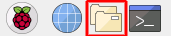
\includegraphics[keepaspectratio,width=5.898cm,height=1.242cm]{text02-img/text02-img001.png}
\flushleft

Figure \stepcounter{Figure}{\theFigure}: フォルダウインドウを開くアイコン}
\end{minipage}

\bigskip
\bigskip
\bigskip

これから作業で使うファイルをコピーしてもらいます。皆さんは、「/home/ユーザー名」のフォルダに、第1回で使うフォルダ「01」をコピーしているはずです。今日は、「02」フォルダをコピーしてから始めます。

まず、「/usr/local/share/ome」という場所を開いてみましょう。

どこにあるか探すことができますか?

わからない時は、TAや先生に聞いてみましょう。

\bigskip
\bigskip

\begin{minipage}{9.781cm}
\centering
{\upshape
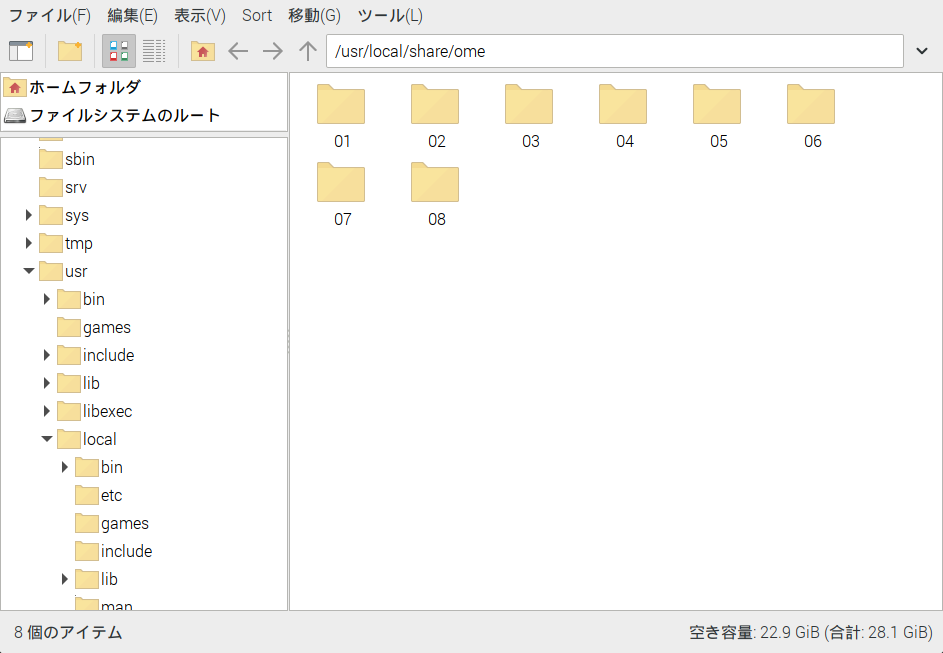
\includegraphics[keepaspectratio,width=11.232cm,height=8.424cm]{text02-img/s_ome02a.png}
\flushleft

Figure \stepcounter{Figure}{\theFigure}: /usr/local/share/ome フォルダ}
\end{minipage}

\bigskip
\bigskip
\bigskip

この中に、「02」という名前のフォルダがあります。これから、この「02」というフォルダを自分の作業フォルダにコピーします。

「02」という名前のフォルダ上でマウスの右クリックを押して「コピー」を選んでください。

\bigskip
\bigskip

\begin{minipage}{9.781cm}
\centering
{\upshape
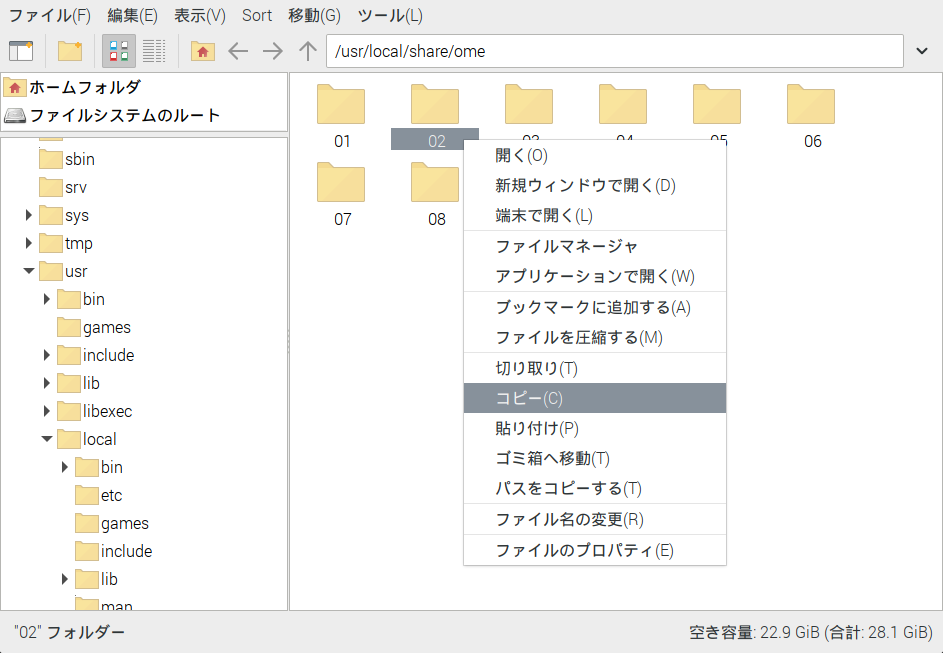
\includegraphics[keepaspectratio,width=11.232cm,height=8.424cm]{text02-img/s_ome02b.png}
\flushleft

Figure \stepcounter{Figure}{\theFigure}: 02フォルダでコピーを選ぶところ}
\end{minipage}

\bigskip
\bigskip
\bigskip

コピーを選ぶだけでは何も起こりません。この後、コピーしたい場所を選びます。

コピー先の場所は、「/home/ユーザー名」のフォルダになります。

たとえば、ユーザー名が「ome」だった場合は、「/home/ome」という場所にコピーします。

コピー先の場所を開いたら、何もない場所でマウスの右クリックを押して「貼り付け」を選んでください。

\bigskip
\bigskip

\begin{minipage}{9.781cm}
\centering
{\upshape
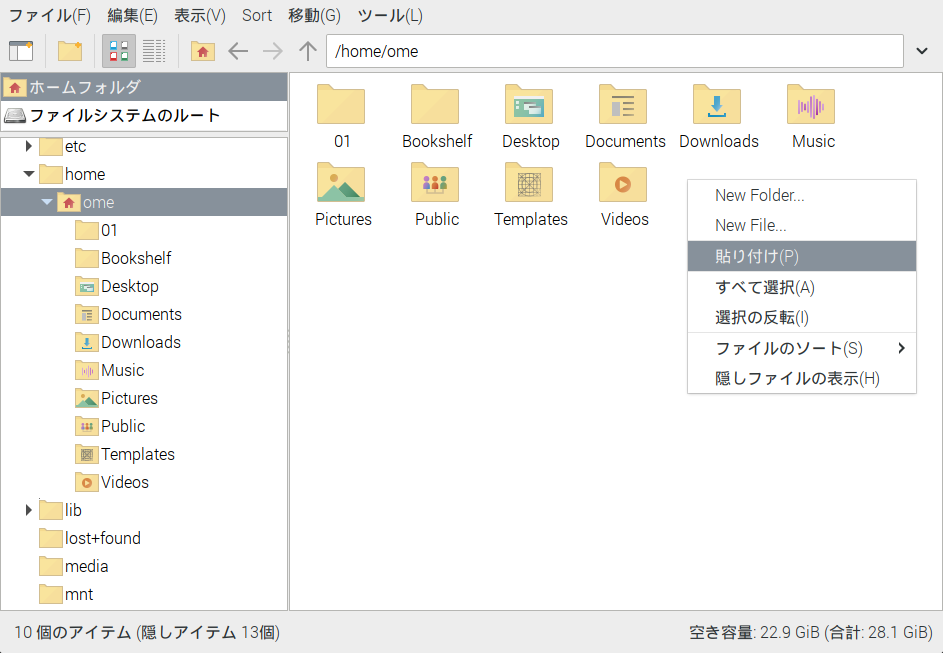
\includegraphics[keepaspectratio,width=11.232cm,height=8.424cm]{text02-img/s_ome02c.png}
\flushleft

Figure \stepcounter{Figure}{\theFigure}: 02フォルダでコピーを選ぶところ}
\end{minipage}

\bigskip
\bigskip
\bigskip

これで先ほどの「/usr/local/share/ome/02」フォルダが、「/home/ユーザー名/02」にコピーされます。

ファイルのコピー、移動、削除などの方法を、よく覚えておきましょう。

ファイルには、画像や文章、音声や動画など、さまざまなデータが入っています。

これから皆さんが作業で使うファイルは、「/home/ユーザー名/02」という場所に置かれています。

ファイルの中身が何なのか、自分が作ったファイルかどうかを知っておいてください。

\bigskip
\bigskip

\begin{minipage}{9.781cm}
\centering
{\upshape
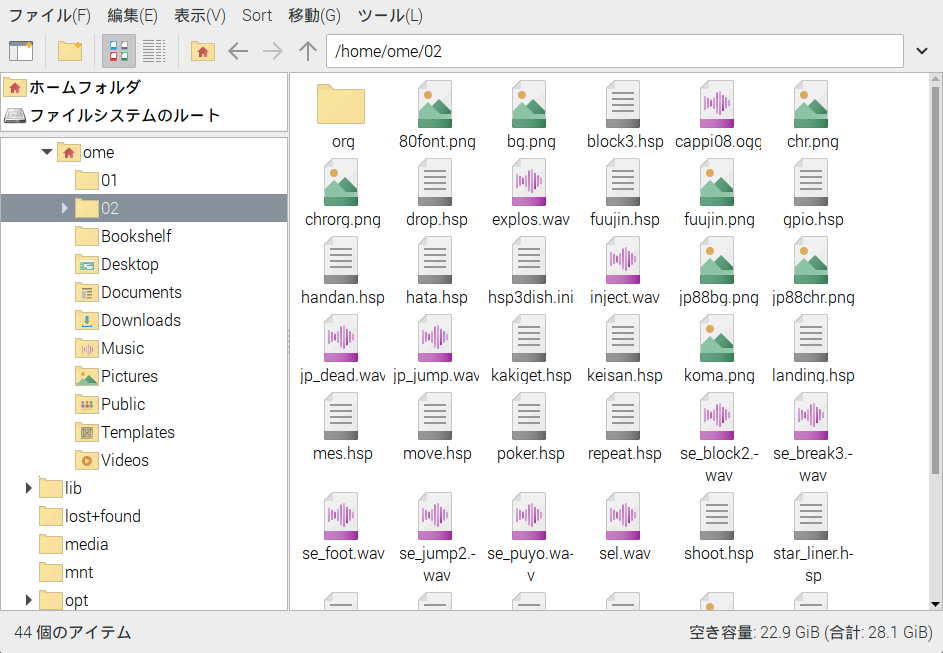
\includegraphics[keepaspectratio,width=11.232cm,height=8.424cm]{text02-img/s_ome02d.png}
\flushleft

Figure \stepcounter{Figure}{\theFigure}: 02フォルダを開いたところ}
\end{minipage}

\bigskip
\bigskip
\bigskip



\clearpage
\subsection{ターミナルの使い方}
\bigskip
\bigskip

これから、Raspberry Piを使って色々なゲームを作ったり、改造したりといった作業をします。
以下の2つに注意しながら、作業を進めていきましょう。

\bigskip

\ \ ・自分が作ったファイル以外は削除や移動しないようにしましょう

\ \ ・ファイルやフォルダはわかりやすい場所に作りましょう


\bigskip
\bigskip

ターミナルの使い方を覚えておきましょう。

ターミナル(コマンドライン)は、キーボードの入力だけでコンピューターをそうさするためのものです。

\bigskip
\bigskip

\begin{minipage}{9.781cm}
\centering
{\upshape

\includegraphics[keepaspectratio,width=7.303cm,height=1.15cm]{text02-img/text02-img003.png}
\flushleft

Figure \stepcounter{Figure}{\theFigure}: ターミナル起動アイコン}
\end{minipage}

\bigskip
\bigskip
\bigskip

ターミナル起動アイコンを選択すると、ターミナル画面のウインドウが開きます。

\bigskip
\bigskip

\begin{minipage}{9.781cm}
\centering
{\upshape
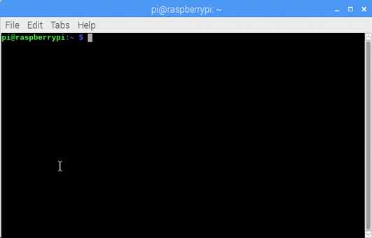
\includegraphics[keepaspectratio,width=9.472cm,height=6.061cm]{text02-img/text02-img004.png}
\flushleft

Figure \stepcounter{Figure}{\theFigure}: ターミナル画面}
\end{minipage}

\bigskip
\bigskip
\bigskip

黒い画面が出てきました。ちょっと難しそうですね。

\bigskip

ターミナルの使い方を覚えておくと、キーボードだけで手早くコンピューターを扱うことができるようになります。

すべての人が必ず使うものではありませんが、とても便利に使うことができるので、少しずつ使って慣れるようにしていきましょう。

\bigskip
\bigskip

たとえば、

\bigskip

\ \ \ \ ls [Enter]

\bigskip

を入力するとファイルの一覧が出てきます。

\bigskip
\bigskip

\begin{minipage}{9.781cm}
\centering
{\upshape
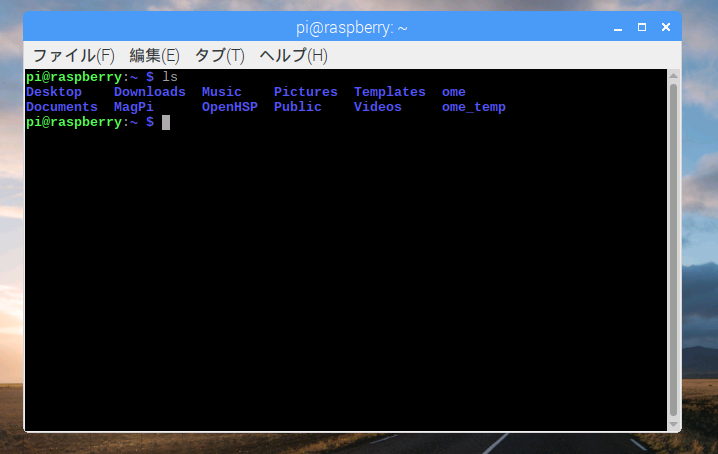
\includegraphics[width=9.71cm,height=6.138cm]{text02-img/text02-img005.png}
\flushleft

Figure \stepcounter{Figure}{\theFigure}: lsコマンドを入力した画面}
\end{minipage}

\bigskip
\bigskip
\bigskip

今回、プログラミングやターミナルなど、キーボードをたくさん使う機会があります。

\bigskip

最初は難しいかもしれませんが、思ったように文字を打つことができるよう、練習をして覚えていきましょう。

\bigskip

キーボードは乱暴に扱わない方がいいですが、間違ったボタンを押したからと言ってコンピューターがこわれることはありません。ですから、間違えることを心配せずに、どんどん自分からキーボードをそうさして、使い方に慣れるよう心掛けてください。

\bigskip

\subsection{プログラミングって何だろう}
\bigskip
\bigskip

皆さんには、プログラミングを初めてもらいます。

プログラミングというのは、プログラムを作ることです。

さて、そもそもプログラムって何でしょう?

パソコンの上で動いている、ワープロソフトやペイントソフト、ゲームなどもみんなまとめて「プログラム」と呼んでいます。


\bigskip

スマホのアプリもプログラムと同じです。ゲーム機のゲームソフトもプログラムです。

「プログラム」というのは自分が考えた通りに動いてくれる予定表のようなものです。

たとえば、学校の授業や運動会にもプログラム(予定表)があり、どんな順番で何をするか決められています。

ビデオレコーダーがテレビ番組を決められた時間に勝手に録画してくれるのもプログラムです。パソコンで動くプログラムは、もっともっと色々な仕事をすばやくこなすことができるものなのです。

\bigskip

・電化製品


\bigskip

家庭で使われている電化製品にも、コンピューターとプログラムが使われています。今では、電気を使うほとんどの機器が、プログラムによって動いています。


\bigskip

・ゲーム機


\bigskip

現在は様々なハードでゲームが遊べるようになっていますが、ビデオゲームは色々な進化をたどってきました。今では、とても高度なコンピューターが使われています。


\bigskip

・ロボットや人工知能


\bigskip

これから大きく発展する分野が、ロボットや人工知能です。これらは、コンピューターと高度なプログラムを組み合わせて作られています。

まだ、簡単なことしかできないロボットが、将来は人間と同じ能力を持って仕事をしているかもしれません。



\bigskip
\bigskip

\begin{minipage}{9.781cm}
\centering
{\upshape
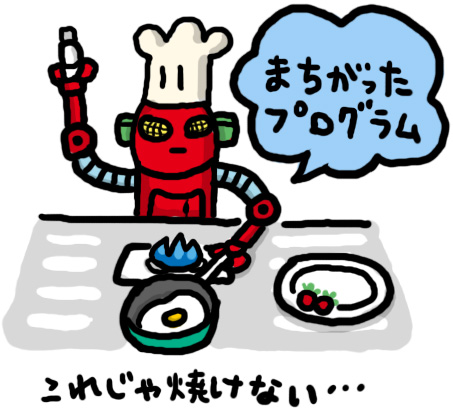
\includegraphics[width=8.031cm,height=7.304cm]{text02-img/text02-img006.jpg}}
\end{minipage}

\bigskip
\bigskip
\bigskip

\bigskip

\clearpage
\subsection{HSPに触れてみよう}
\bigskip
\bigskip

それでは、さっそくプログラム作りを始めてみましょう。
プログラムを作ったり、打ち込んだりすることをプログラミングといいます。
これから、やることの内容はつぎの通りです。

\bigskip

\begin{itemize}
\item {\bfseries
プログラムの呼び出し方と動かし方を覚える}
\item {\bfseries
センサーボードを使って仕組みを覚える}
\item {\bfseries
プログラムを自分の手で実際に打ち込んでみること}
\item {\bfseries
ゲームを改造して自分だけのオリジナルゲームにすること}
\end{itemize}

\bigskip

プログラムを覚えたら、何ができるのか?

そして、プログラムを覚えておくと将来どんないいことがあるのか?

皆さんもプログラムの世界について学んでいきましょう。

今回みなさんに使ってもらうのは「ホットスーププロセッサ ( Hot Soup Processor )」、りゃくして「HSP(エッチ・エス・ピー)」と呼ばれているツールです。ゲームを作るのに向いているだけでなく、小中学生にも使えるくらい簡単で、参考になる本もいっぱい出ています。


\bigskip

\bigskip

左上のRaspberry Piメニューの「プログラミング」項目に、「HSP Script Editor」(HSPスクリプトエディタ)という項目があるはずです。

メニューを開いて確認(かくにん)してみましょう。

\bigskip
\bigskip

\begin{minipage}{9.781cm}
\centering
{\upshape
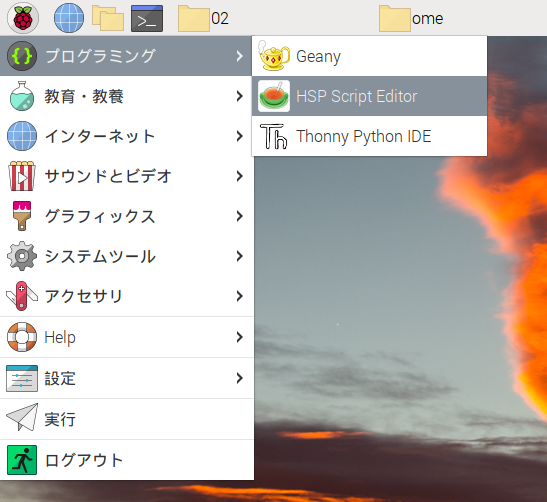
\includegraphics[keepaspectratio,width=7.31cm,height=6.562cm]{text02-img/s_hspmenu.png}
\flushleft

Figure \stepcounter{Figure}{\theFigure}: プログラミング項目のメニュー}
\end{minipage}

\bigskip
\bigskip
\bigskip

「HSP Script Editor」のアイコンをクリックして起動させてみましょう。
Raspberry Piメニューからでも、ターミナルから「hsed」と打ち込んでも起動させることができるので覚えておきましょう。
\bigskip
\bigskip

\begin{minipage}{9.781cm}
\centering
{\upshape
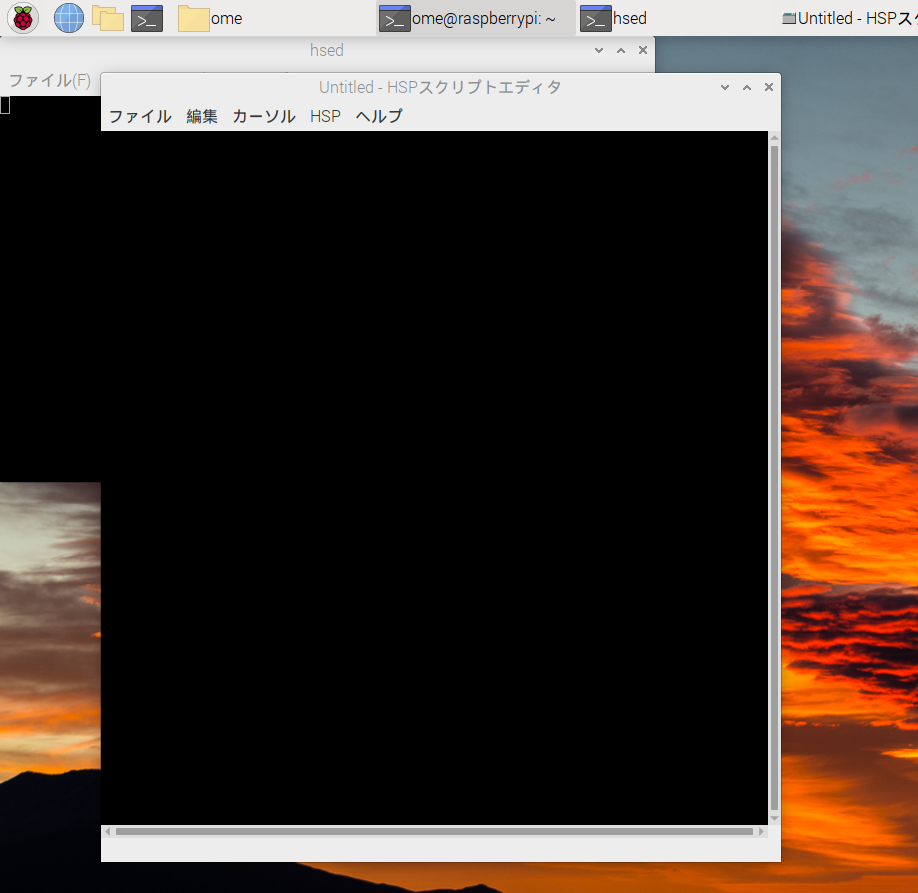
\includegraphics[keepaspectratio,width=7.31cm,height=6.562cm]{text02-img/s_hsed.png}
\flushleft

Figure \stepcounter{Figure}{\theFigure}: HSPスクリプトエディタを起動したところ}
\end{minipage}

\bigskip
\bigskip
\bigskip

「HSPスクリプトエディタ」は、テキストエディタ(MousePad)と同じように好きな文字を打ち込むことができます。文字を直したり、カーソルを好きな場所に移動したりする方法がわからない人は、近くの先生に聞いてみてください。


\bigskip

実際にできあがっているプログラムを見てみましょう。

ファイル→「開く」メニューから /home/ユーザー名/02 フォルダの中にある「shoot.hsp」を読み込んでください。

作業は、すべて「/home/ユーザー名/02」フォルダで行ないます。

見つからない場合は、まわりの友達か、近くの先生に聞いてみてください。

\bigskip
\bigskip

\begin{minipage}{9.781cm}
\centering
{\upshape
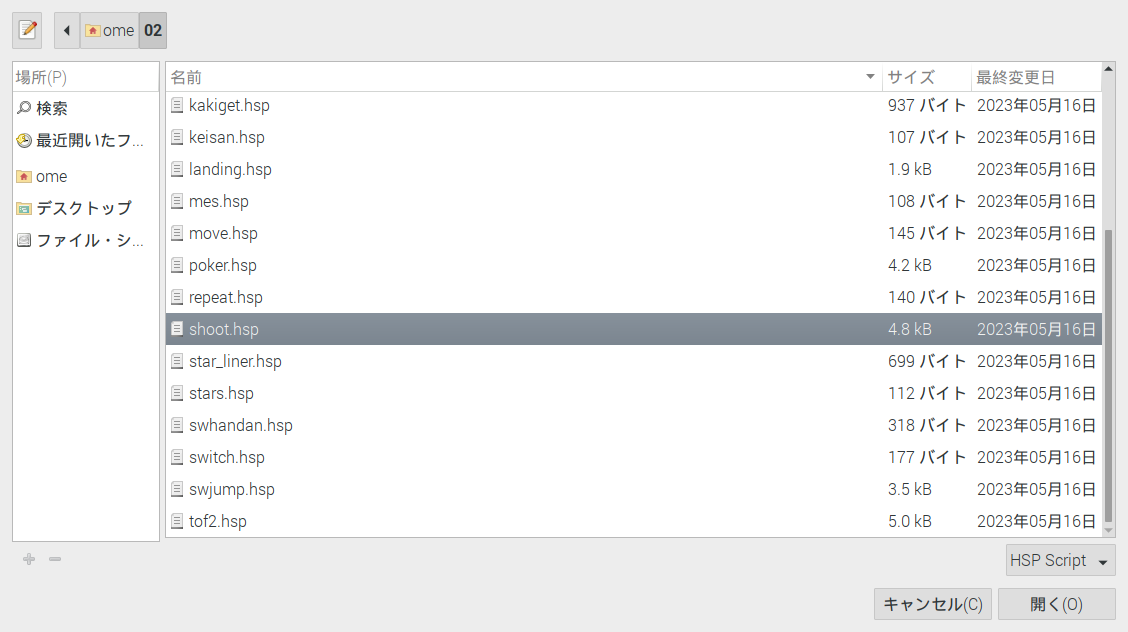
\includegraphics[keepaspectratio,width=7.31cm,height=6.562cm]{text02-img/s_openfolder.png}
\flushleft

Figure \stepcounter{Figure}{\theFigure}: フォルダから読み込む画面}
\end{minipage}

\bigskip
\bigskip
\bigskip

だらだらと長い文字が読み込まれましたか?

今は意味がわからなくても大丈夫です。

まずは、[F5]キーを押して動かしてみましょう。[F5]キーを押すと読み込まれたスクリプトをもとにプログラムがうごきだします。

\bigskip

\clearpage
\subsection{シューティングゲームの遊び方}

\bigskip
\bigskip

\ \ 1.
タイトル画面で[Enter]キーを押すとゲームがスタートします

\ \ 2.
カーソルキーで上下左右に移動、ミサイルは自動発射です

\ \ 3.
敵や弾に当たるとゲームオーバーになってしまいます


\bigskip
\bigskip

\begin{minipage}{9.781cm}
\centering
{\upshape
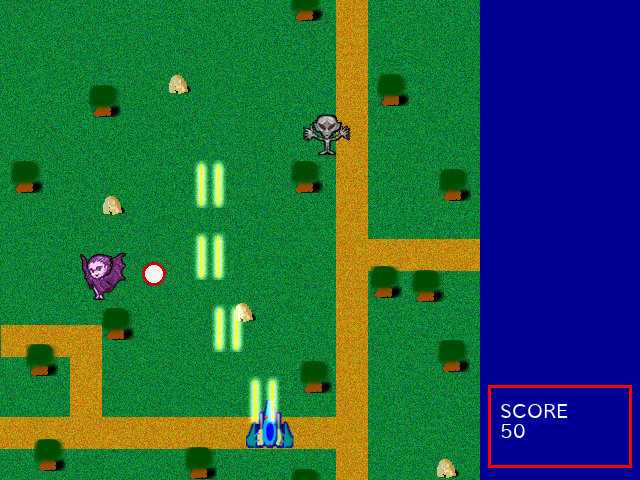
\includegraphics[keepaspectratio,width=7.31cm,height=6.562cm]{text02-img/s_shoot.png}
\flushleft

Figure \stepcounter{Figure}{\theFigure}: シューティングゲームの画面}
\end{minipage}

\bigskip
\bigskip
\bigskip

ゲームを遊び終わったらウインドウ右上の「×」を押してウィンドウを閉じましょう

\bigskip
\bigskip

\begin{minipage}{9.781cm}
\centering
{\upshape
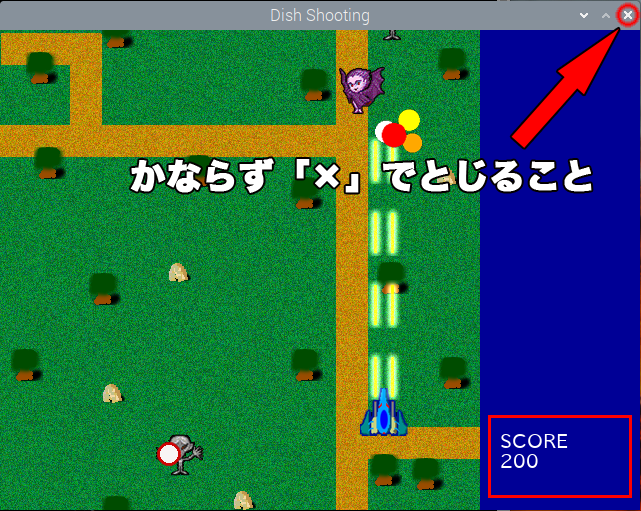
\includegraphics[keepaspectratio,width=7.31cm,height=6.562cm]{text02-img/s_shoot2.png}
\flushleft

Figure \stepcounter{Figure}{\theFigure}: ウインドウを閉じるボタン}
\end{minipage}

\bigskip
\bigskip
\bigskip

このようにスクリプトがあればゲームを動かすことができます。

ゲームが終わったら、かならず「×」ボタンを押してエディタの画面に戻ってください。「×」ボタンを押さないと、スクリプトエディタのそうさに戻ることができません。

さて、このスクリプトエディタに表示されている長い文章のことを「スクリプト」と呼びます。「プログラム」は、できあがったもの全体を指してまぎらわしいので、プログラミングで打ち込むための言葉は「スクリプト」と呼ぶようにしますので覚えておいてください。


\bigskip

HSPスクリプトエディタは、打ち込まれたスクリプトを[F5]キーで実行する機能、そのスクリプトを.hspファイルとして保存したり読み込んだりする機能があります。

実行された時には、新しいウインドウに表示され、右上の[×]ボタンを押すことで、元の編集画面に戻ります。

\bigskip
\bigskip

\begin{minipage}{9.781cm}
\centering
{\upshape

\includegraphics[width=15.533cm,height=4.86cm]{text02-img/text02-img013.png}}
\end{minipage}

\bigskip
\bigskip
\bigskip

HSPスクリプトエディタの基本的な使い方をよく覚えておきましょう。

スクリプトを書けるようになると、画面の絵や音、そしてハードウェアなど様々なデバイスを組み合わせて、あなたの考えたプログラムを作ることができるようになります。

\bigskip

\subsection{例題に挑戦しよう}

\bigskip
\bigskip

ここまで終わってしまった人は、以下の例題にも挑戦してみよう。


\bigskip

・ターミナルからHSPスクリプトエディタを起動する

・ドロップパズル(drop)を読み込んで動かす

・ブロック崩し(block3)を読み込んで動かす

・その他のゲームでラズパイに親しむ


\bigskip

例題の考え方がわからない時は、近くのTAか先生に聞いてください。

わからない所は、そのままにせず、必ず答えを見つけてから先に進みましょう。

\bigskip


\clearpage
\subsection{例題1 HSPスクリプトエディタをターミナルから起動する}
\bigskip
\bigskip

{\bfseries
考え方}


\bigskip

ターミナルからHSPスクリプトエディタを起動してみましょう。

HSPスクリプトエディタを起動するためのコマンドは、「hsed」です。

\bigskip

{\bfseries
例題1 答え}


\bigskip

プログラムを打ち込むためには、「HSPスクリプトエディタ」というツールを使うことを覚えました。

Raspberry Piメニューにある「HSP Script
Editor」のアイコンをクリックして起動させることができるほか、ターミナルからhsedコマンドで直接起動させることもできます。

\bigskip

ターミナル起動アイコンを選択すると、ターミナル画面のウインドウが開きます。

\bigskip
\bigskip

\begin{minipage}{9.781cm}
\centering
{\upshape
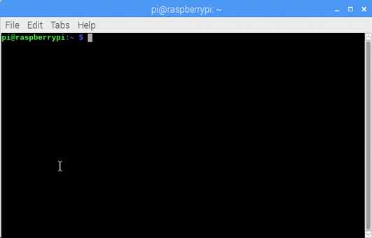
\includegraphics[keepaspectratio,width=8.52cm,height=5.45cm]{text02-img/text02-img004.png}
\flushleft

Figure \stepcounter{Figure}{\theFigure}: ターミナル画面}
\end{minipage}

\bigskip
\bigskip
\bigskip

ターミナルの画面で

{\bfseries
hsed [Enter]}

\bigskip

と入力しましょう。

HSPスクリプトエディタが起動することを確認(かくにん)してください。


\clearpage
\subsection{例題2 ドロップパズル(drop)を読み込んで動かす}
\bigskip
\bigskip

{\bfseries
考え方}

\bigskip


\bigskip

HSPスクリプトエディタからスクリプト(プログラム)を読み込む方法と、実行する方法を思い出してみてください。

それでは、HSPスクリプトエディタからドロップパズル(drop.hsp)を読み込んで遊んでみましょう。

ドロップパズル(drop.hsp)は、/home/ユーザー名/02のフォルダにあります。

\bigskip

\bigskip

{\bfseries
例題2 答え}

\bigskip

HSPスクリプトエディタの基本的な使い方をよく覚えておきましょう。

\bigskip
\bigskip

\begin{minipage}{9.781cm}
\centering
{\upshape

\includegraphics[keepaspectratio,width=15.533cm,height=4.86cm]{text02-img/text02-img013.png}}
\end{minipage}

\bigskip
\bigskip
\bigskip

このように、HSPスクリプトエディタは、打ち込まれたスクリプトを[F5]キーで実行する機能、そのスクリプトを.hspファイルとして保存したり読み込んだりする機能があります。

実行した後には、ウインドウの「×」ボタンを押して元の画面に戻ります。

\bigskip

ファイル→「開く」メニューから/home/ユーザー名/02のフォルダに移動してから、「drop.hsp」を読み込んでみましょう。

\bigskip
\bigskip

\begin{minipage}{9.781cm}
\centering
{\upshape
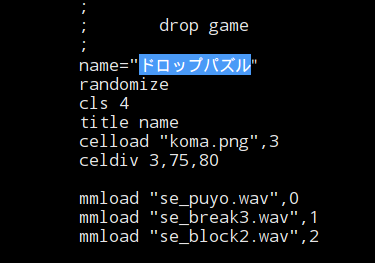
\includegraphics[keepaspectratio,width=9.049cm,height=6.346cm]{text02-img/text02-img014.png}
\flushleft

Figure \stepcounter{Figure}{\theFigure}: ドロップパズルのスクリプト}
\end{minipage}

\bigskip
\bigskip
\bigskip

読み込まれたら、[F5]キーで実行します。

\bigskip
\bigskip

\begin{minipage}{9.781cm}
\centering
{\upshape
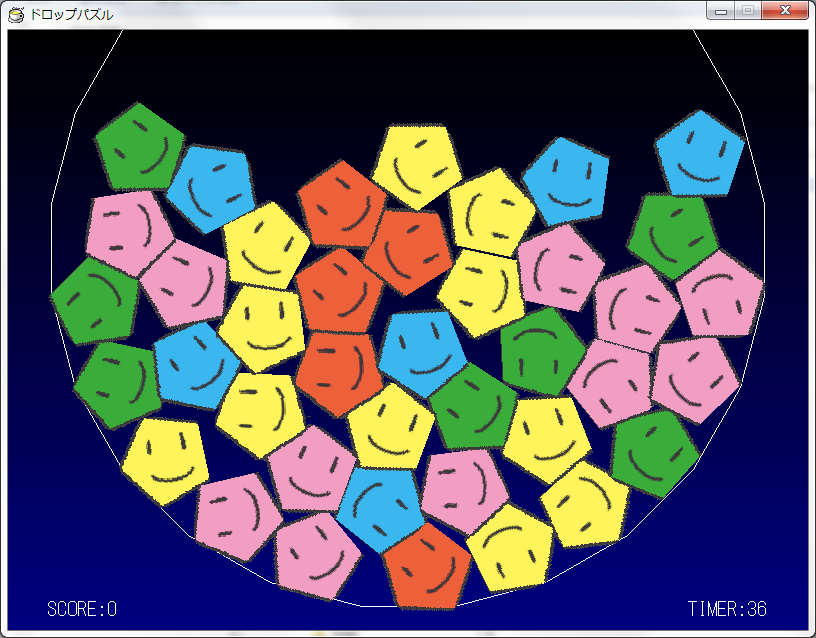
\includegraphics[keepaspectratio,width=10.605cm,height=8.306cm]{text02-img/text02-img015.png}
\flushleft

Figure \stepcounter{Figure}{\theFigure}: ドロップパズルゲームの画面}
\end{minipage}

\bigskip
\bigskip
\bigskip

ドロップパズルは、上から落ちてくる5角形のパネルをうまく消していくゲームです。

パネルの上にマウスカーソルを合わせて、ボタンを押しながら同じ色のパネルをなぞってください。

すると、同じ色のパネルが消えて、新しいパネルが上から降ってきます。

一度に同じ色のパネルをたくさん消すと、高いスコアがもらえます。

時間内にできるだけ高いスコアを出せるように頑張ってください。

\bigskip

ゲームを終了する時は、ウインドウの「×」ボタンを押してください。


\clearpage
\subsection{例題3 ブロック崩し(block3)を読み込んで動かす}
\bigskip
\bigskip

{\bfseries
考え方}

\bigskip


\bigskip

/home/ユーザー名/02のフォルダにある他のスクリプトを実行してみましょう。

「block3.hsp」は、ブロック崩しゲームのスクリプトです。

ドロップパズルと同じように読み込んで動かしてみましょう。

\bigskip

\bigskip

{\bfseries
例題3 答え}

\bigskip

ファイル→「開く」メニューから/home/ユーザー名/02のフォルダに移動してから、「block3.hsp」を読み込んでみましょう。

読み込まれたら、[F5]キーで実行します。


\bigskip

マウスをうまく動かしてラケットをそうさします。ボールを打ち返してブロックを崩してください。

ボールが下まで落ちてしまうとアウトです。

\bigskip
\bigskip

\begin{minipage}{9.781cm}
\centering
{\upshape
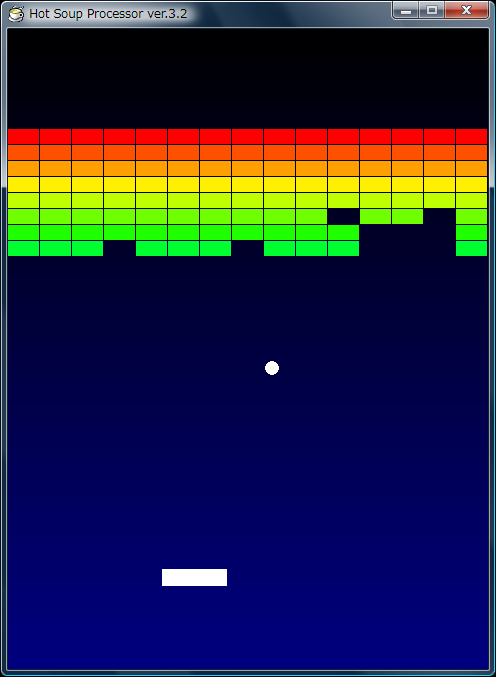
\includegraphics[keepaspectratio,width=8.467cm,height=7.17cm]{text02-img/text02-img016.png}
\flushleft

Figure \stepcounter{Figure}{\theFigure}: ブロック崩しの画面}
\end{minipage}

\bigskip
\bigskip
\bigskip

ゲームを終了する時は、ウインドウの「×」ボタンを押してください。


\clearpage
\subsection{例題4 重力ゲーム(tof2)を読み込んで動かす}
\bigskip
\bigskip

{\bfseries
考え方}

\bigskip


\bigskip

/home/ユーザー名/02のフォルダにある他のスクリプトを実行してみましょう。

「tof2.hsp」は、重力ゲームのスクリプトです。

ドロップパズルと同じように読み込んで動かしてみましょう。

\bigskip
\bigskip

\begin{minipage}{9.781cm}
\centering
{\upshape
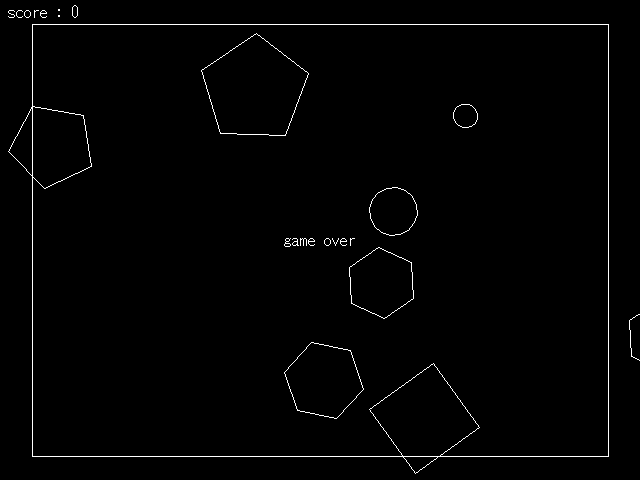
\includegraphics[keepaspectratio,width=8.467cm,height=7.17cm]{text02-img/s_tof2.png}
\flushleft

Figure \stepcounter{Figure}{\theFigure}: tof2の画面}
\end{minipage}

\bigskip
\bigskip
\bigskip

ゲームを終了する時は、ウインドウの「×」ボタンを押してください。

\bigskip

\bigskip

{\bfseries
例題4 答え}

\bigskip

カーソルキーで大きな円をうまく動かして小さい円をバウンドさせます。
小さい円で敵を攻撃することができます。できるだけ多くの敵を倒してください。

\bigskip

ゲームを終了する時は、ウインドウの「×」ボタンを押してください。


  % Sensor:

\clearpage
\section{センサーボードを使ってみよう}
\subsection{センサーボードって何だろう}
\bigskip
\bigskip

プログラムによって、画面の上でゲームが遊べることがわかりました。

これはちょうどスマートフォンや家庭用ゲーム機でゲームを遊ぶのと似ています。

今回、皆さんが使うRaspberryPiは、ゲームだけでなく明るさや温度などさまざまな情報を調べることのできるセンサーボードを接続することができます。

\bigskip
\bigskip

\begin{minipage}{9.781cm}
\centering
{\upshape
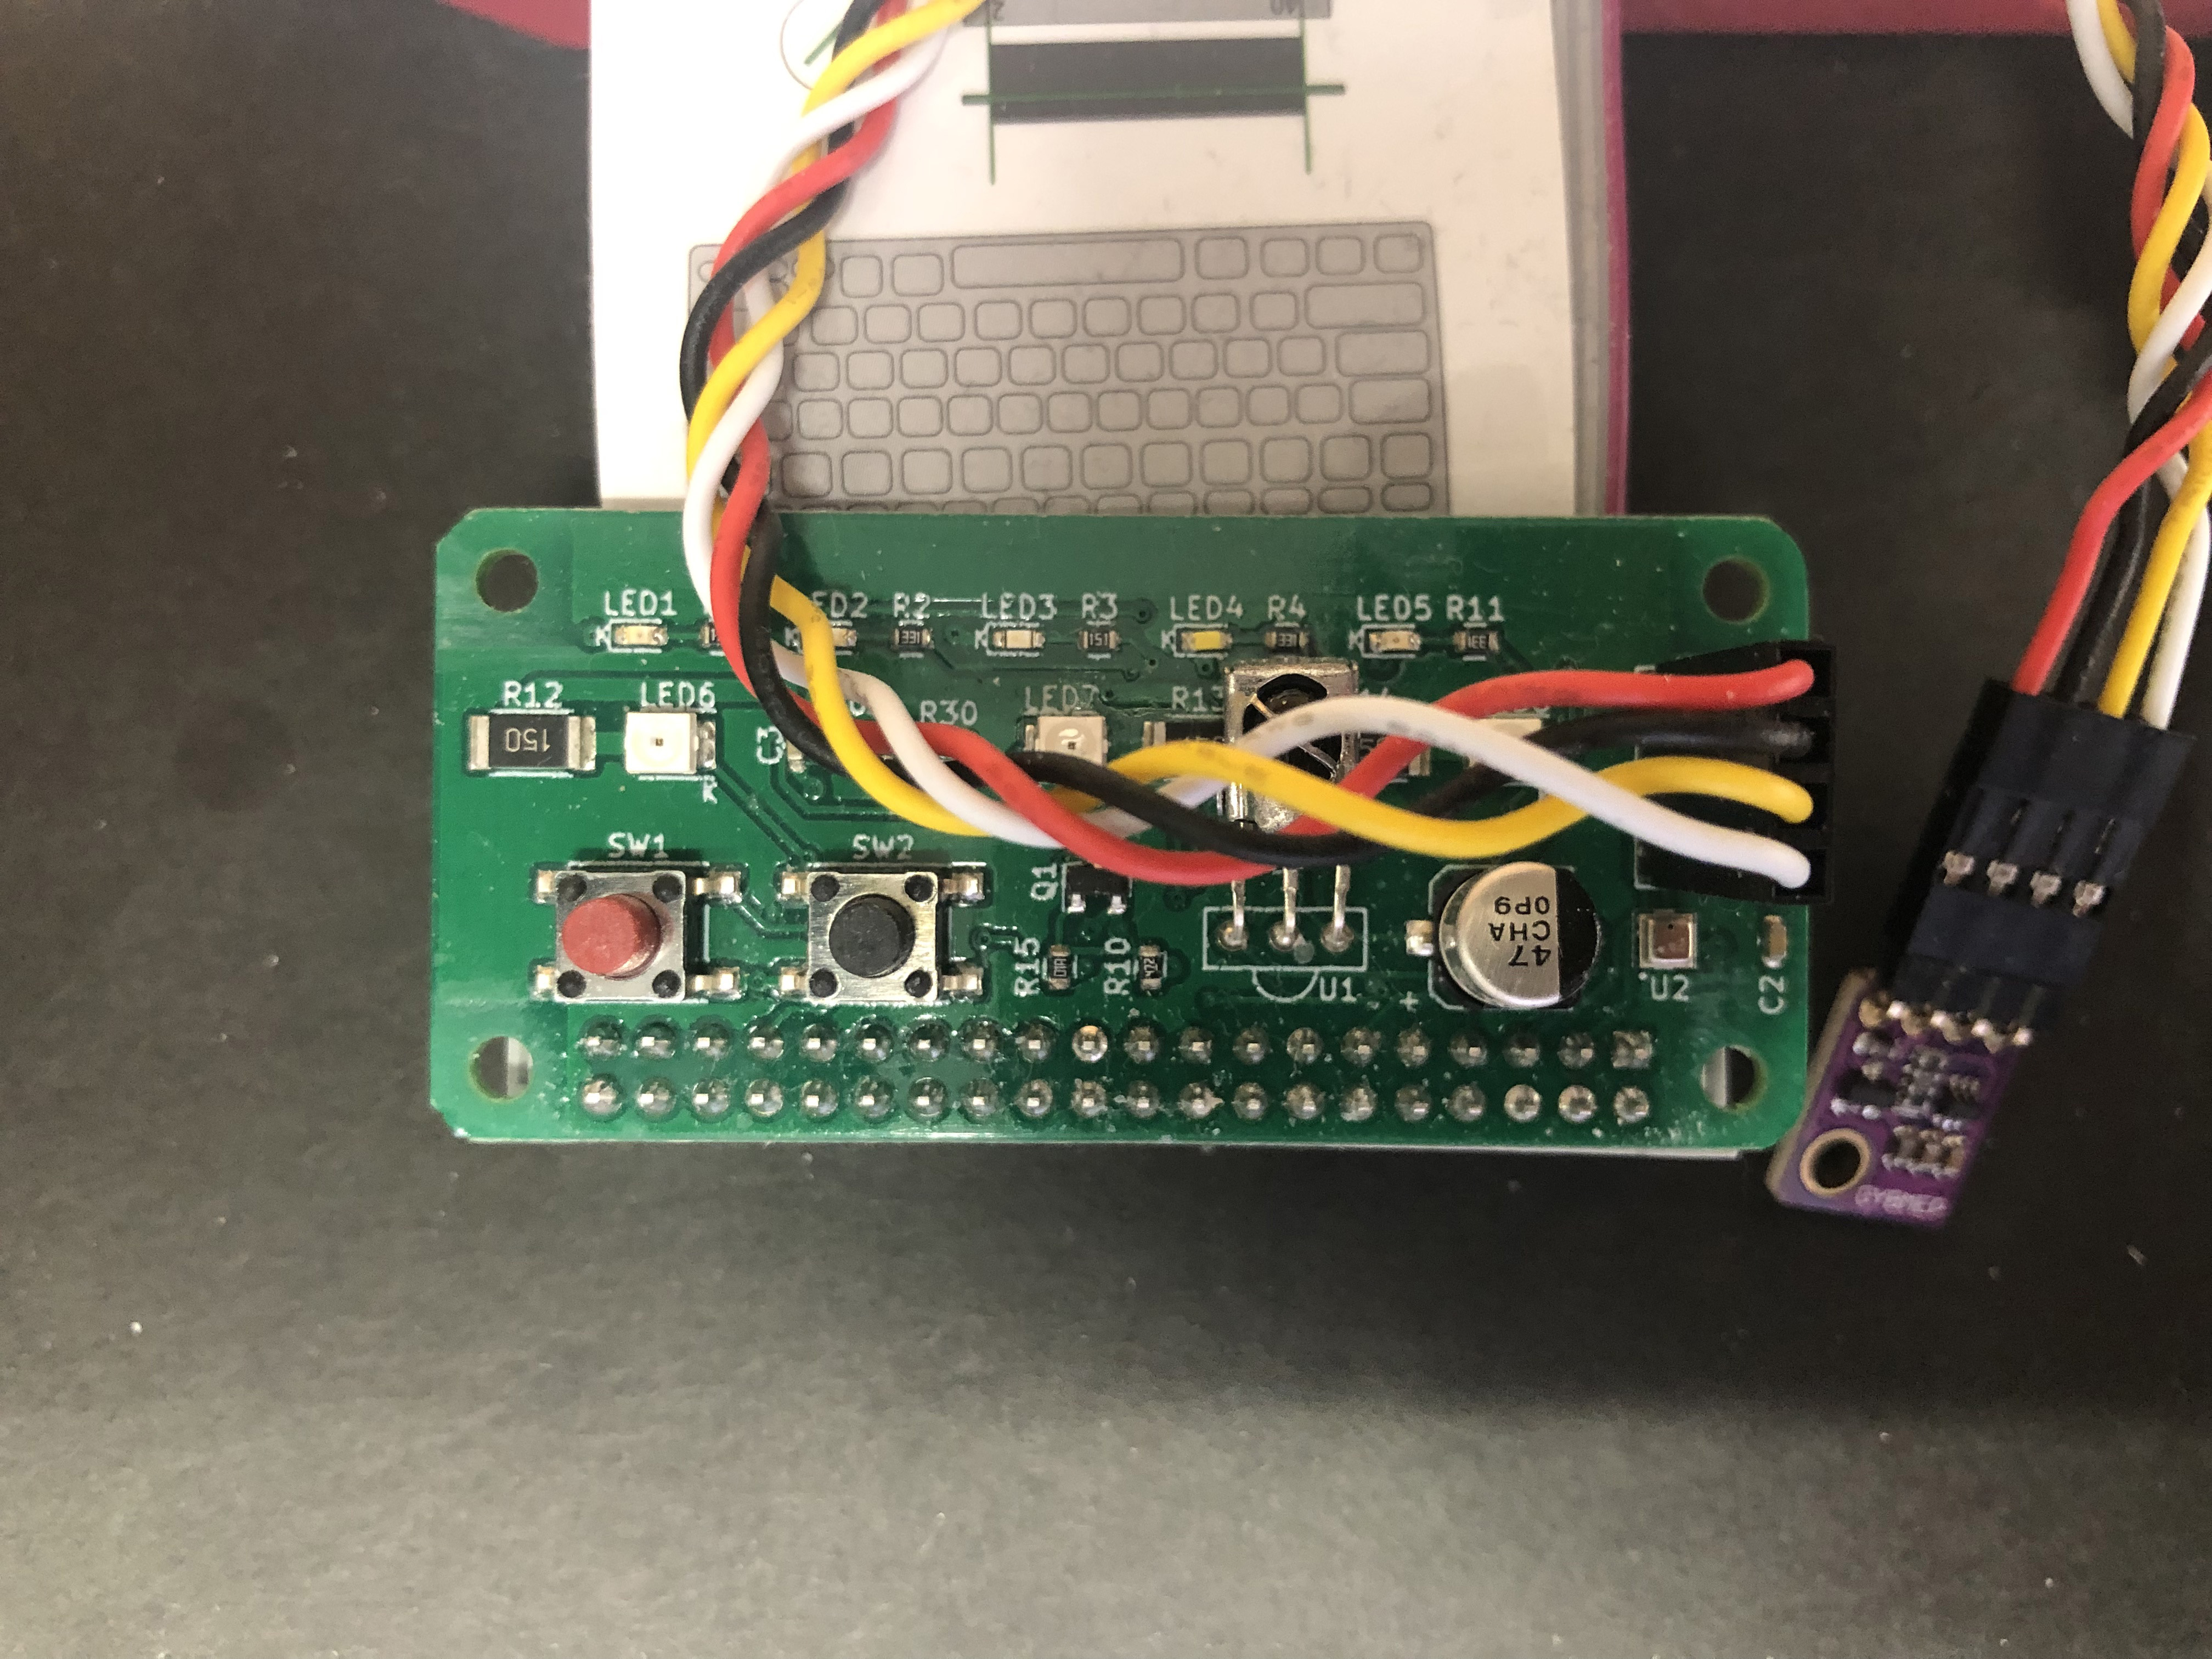
\includegraphics[keepaspectratio,width=9.79cm,height=7.955cm]{text02-img/sensor1.jpg}
\flushleft

Figure \stepcounter{Figure}{\theFigure}: センサーボード}
\end{minipage}

\bigskip
\bigskip
\bigskip

まず最初にRaspberryPiとセンサーボードを接続しましょう。

普通の電気製品は、ケースや保護がありますが、センサーボードやRaspberryPiは、回路の基板そのままの状態です。
触っても感電することはありませんが、静電気によってこわれたりケガをすることがあるので、回路部分を触らないように注意しましょう。

\bigskip
\bigskip

\begin{minipage}{9.781cm}
\centering
{\upshape
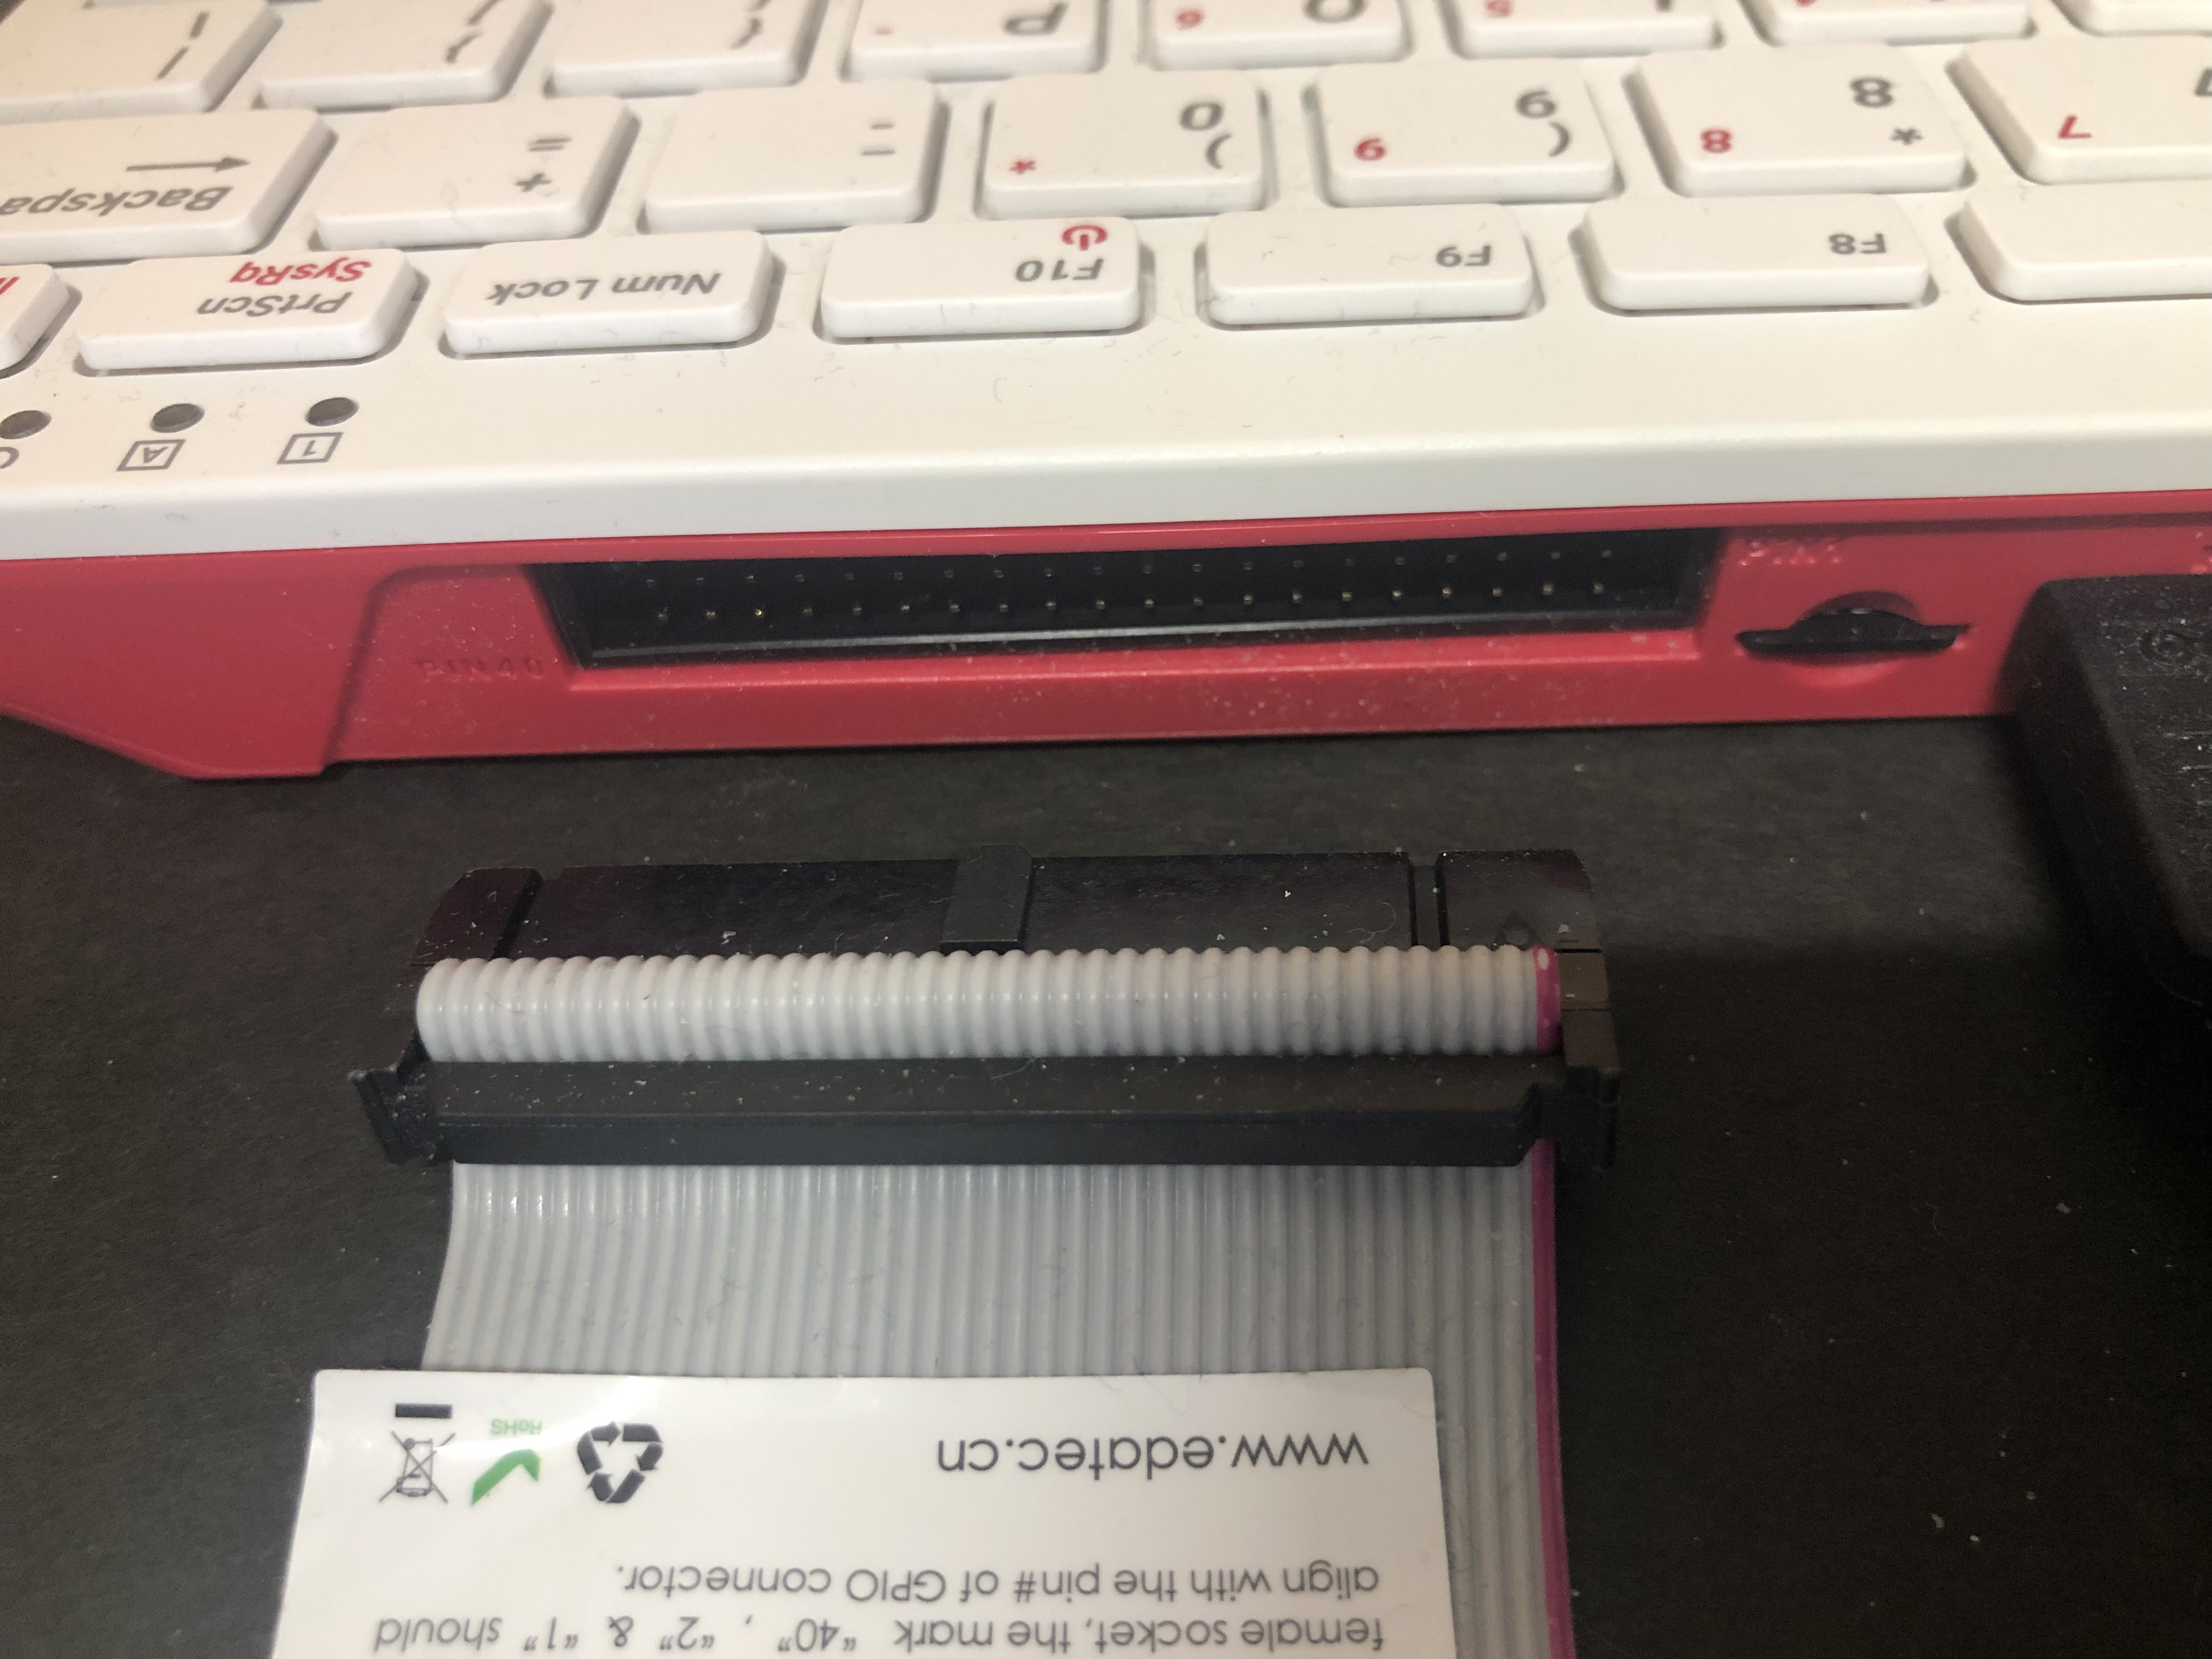
\includegraphics[keepaspectratio,width=9.79cm,height=7.955cm]{text02-img/sensor2.jpg}
\flushleft

Figure \stepcounter{Figure}{\theFigure}: 接続コネクタと拡張ケーブル}
\end{minipage}

\bigskip
\bigskip
\bigskip

RaspberryPiの裏がわに、拡張ケーブルを差し込むための接続コネクタがあるのを確認(かくにん)してください。

拡張ケーブルにセンサーボードをつなげます。ピンの位置がずれたり、さかさまに差さないように注意してください。

正しく差し込まれたことを先生やTAに必ず見てもらってください。

\bigskip
\bigskip

\begin{minipage}{9.781cm}
\centering
{\upshape
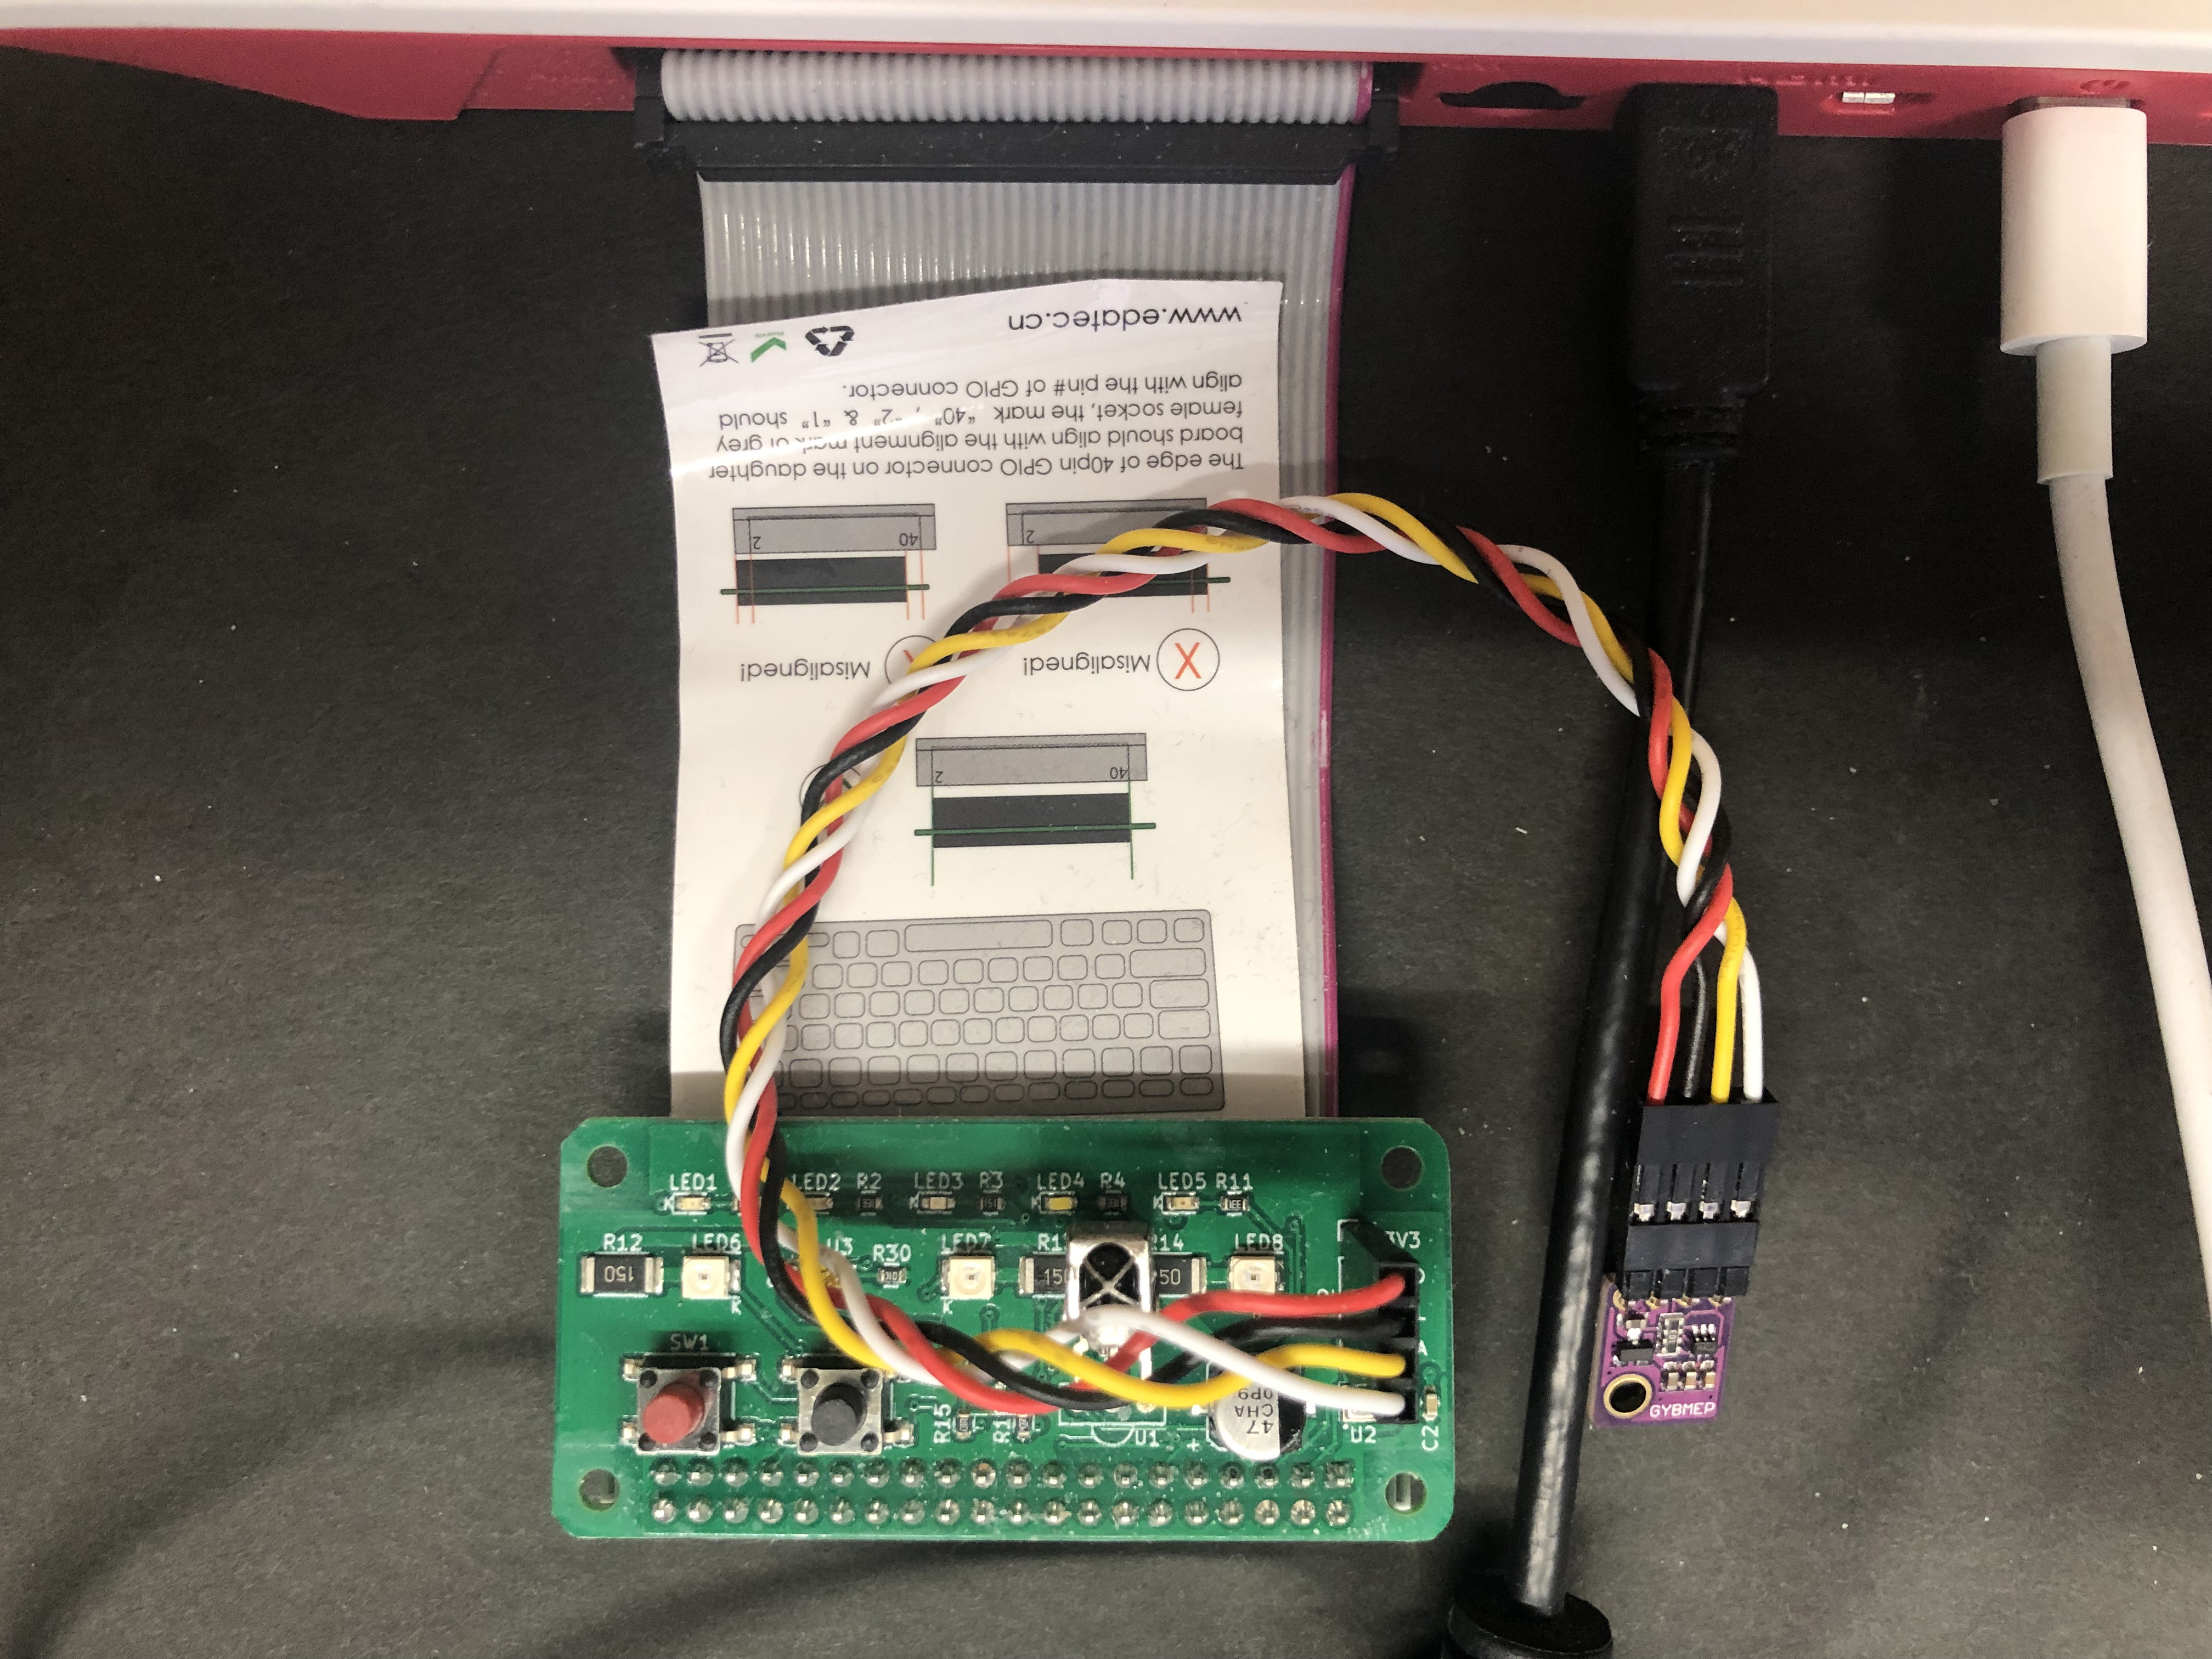
\includegraphics[keepaspectratio,width=9.79cm,height=7.955cm]{text02-img/sensor3.jpg}
\flushleft

Figure \stepcounter{Figure}{\theFigure}: 拡張ケーブルを差し込んだところ}
\end{minipage}

\bigskip
\bigskip
\bigskip

次にRaspberryPi本体に、拡張ケーブルを差し込みます。

きちんと奥まで差し込まれていることを確認(かくにん)しましょう。

\bigskip
\bigskip

\begin{minipage}{9.781cm}
\centering
{\upshape
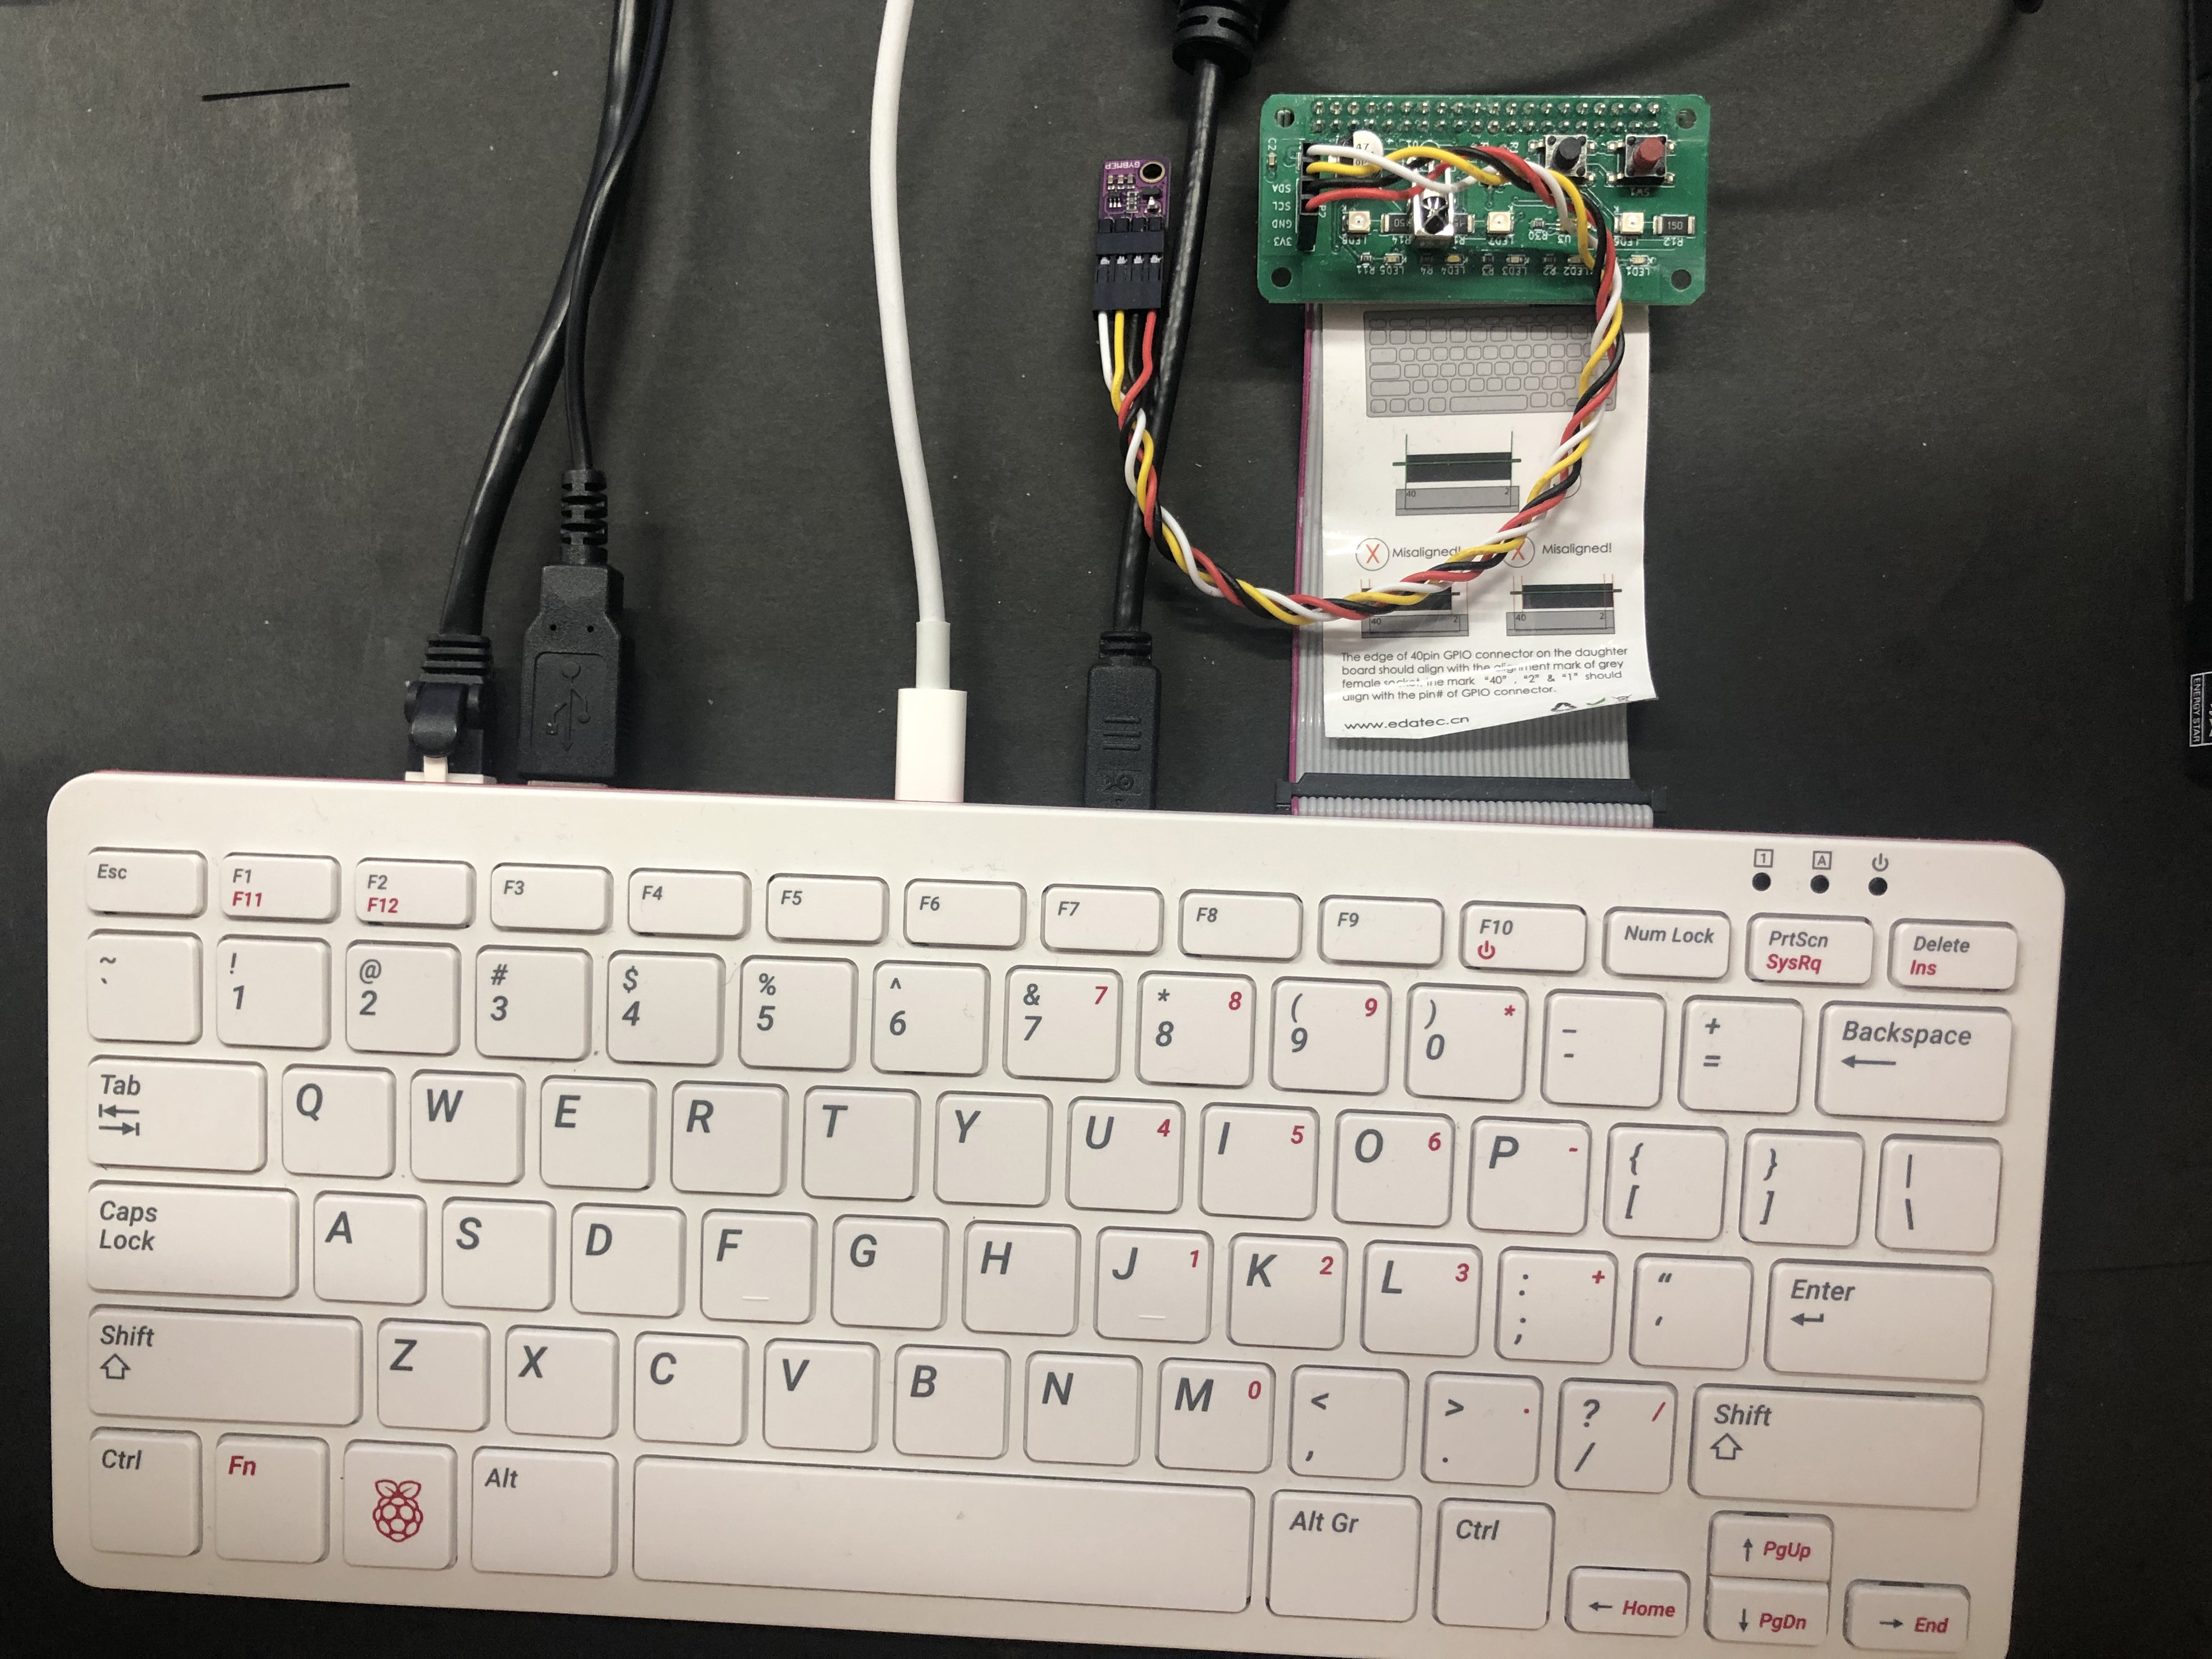
\includegraphics[keepaspectratio,width=9.79cm,height=7.955cm]{text02-img/sensor4.jpg}
\flushleft

Figure \stepcounter{Figure}{\theFigure}: Raspberry Piとセンサーボード}
\end{minipage}

\bigskip
\bigskip
\bigskip

これで、接続されたセンサーボードを使ったプログラムが動くようになります。

プログラミングは、画面を動かすだけでなく、RaspberryPiが持つすべての機能を自由に組み合わせて使うことができるのです。

\bigskip

それでは、さっそくプログラミングを始めてみましょう。

これから、やることの内容はつぎの通りです。


\bigskip

{\bfseries
・LEDがてんめつするスクリプト(gpio)を読み込んで動かす}

{\bfseries
・メッセージが出るスクリプト(mes)を改造してみる}

{\bfseries
・エディタの編集について覚える}

{\bfseries
・別なLEDを光らせてみよう}

{\bfseries
・別なメッセージを出してみよう}

{\bfseries
・改造したスクリプトを保存してみよう}

{\bfseries
・命令とパラメーターを覚えよう}


\clearpage
\subsection{プログラムとスクリプト}
\bigskip
\bigskip

プログラムを打ち込むためには、「HSPスクリプトエディタ」というツールを使うことを覚えました。

このエディタに打ち込む言葉のことを「スクリプト」と呼んでいることを覚えていますか?

スクリプトは、プログラムがどのように動くかを書いた設計図のようなものです。これは、ソースコードとも呼ばれています。

皆さんが使っているアプリやゲーム、パソコンのプログラムもソースコードをもとにして作られています。

スクリプトエディタは、スクリプトを書いて実行するためのツールです。


\bigskip


\bigskip

スクリプトは、プログラムを作るための元になるものですが、その書き方には色々な種類があります。

これは英語とも日本語とも違う特別なルールを持った言葉です。この言葉は「プログラム言語」と呼ばれていて、やりたいことに合わせて色々な種類があります。

\bigskip
\bigskip

\begin{minipage}{9.781cm}
\centering
{\upshape
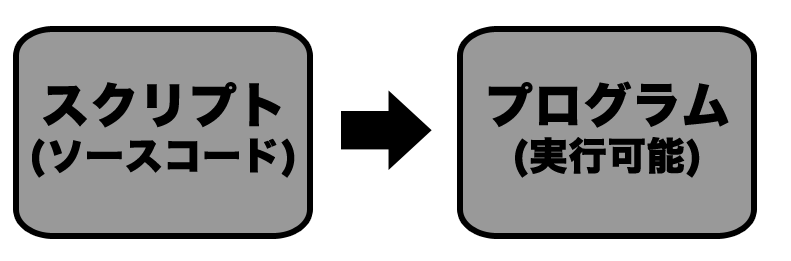
\includegraphics[keepaspectratio,width=11.509cm,height=3.803cm]{text02-img/text02-img022.png}}
\end{minipage}

\bigskip
\bigskip
\bigskip

今回、皆さんが使うHSPは小文字のアルファベット(英語)でスクリプトを打ち込みます。でも英語を知らなくても構いません。漢字変換がいらないので、慣れれば英語の方が打ち込むのが早くなりますし、世界中の人が同じ方法で打ち込んでいるので、今覚えておけば将来にも役立つはずです。


\bigskip


\clearpage
\subsection{LEDがてんめつするスクリプト}
\bigskip
\bigskip

かんたんなスクリプトを読み込んでみます。

前の時間と同様に、ファイル→「開く」メニューから「gpio.hsp」を読み込んでから、「F5」キーを押して実行してみましょう。

センサーボードのLEDがてんめつしていたら成功です。うまくいかない人は、となりの友だちか、近くの先生に見てもらいましょう。

\bigskip
\bigskip

\begin{minipage}{9.781cm}
\centering
{\upshape
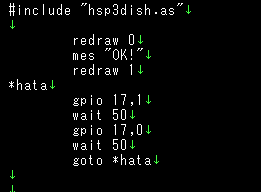
\includegraphics[keepaspectratio,width=8.387cm,height=6.17cm]{text02-img/text02-img023.png}
\flushleft

Figure \stepcounter{Figure}{\theFigure}: gpio.hspのスクリプト}
\end{minipage}

\bigskip
\bigskip
\bigskip

正しく動いたのを確認(かくにん)したらウインドウの「×」ボタンを押して画面を閉じましょう。


\bigskip

\ \ (HSPのルール)


\bigskip

\ \ スクリプトエディタに打ち込んだ通りに動く

\ \ 動かす時は[F5]キーを押す

\ \ 確認(かくにん)したらウインドウの「×」ボタンを押して画面を閉じる


\bigskip

スクリプトを見てみましょう。

英単語の後に数字書かれているものが何行も書かれています。

最初はまったく意味がわからないですね。

\bigskip

最初の行にある


\bigskip

\ \ \#include “hsp3dish.as”


\bigskip

は、最初に書いておくおまじないのようなものと考えておいてください。

RaspberryPiを使う時には、最初にこの1行を入れておくことを覚えておきましょう。


\bigskip

HSPのスクリプトは、英文字による「命令」と数字などによる「パラメーター」によって作られています。

\bigskip
\bigskip

\begin{minipage}{9.781cm}
\centering
{\upshape
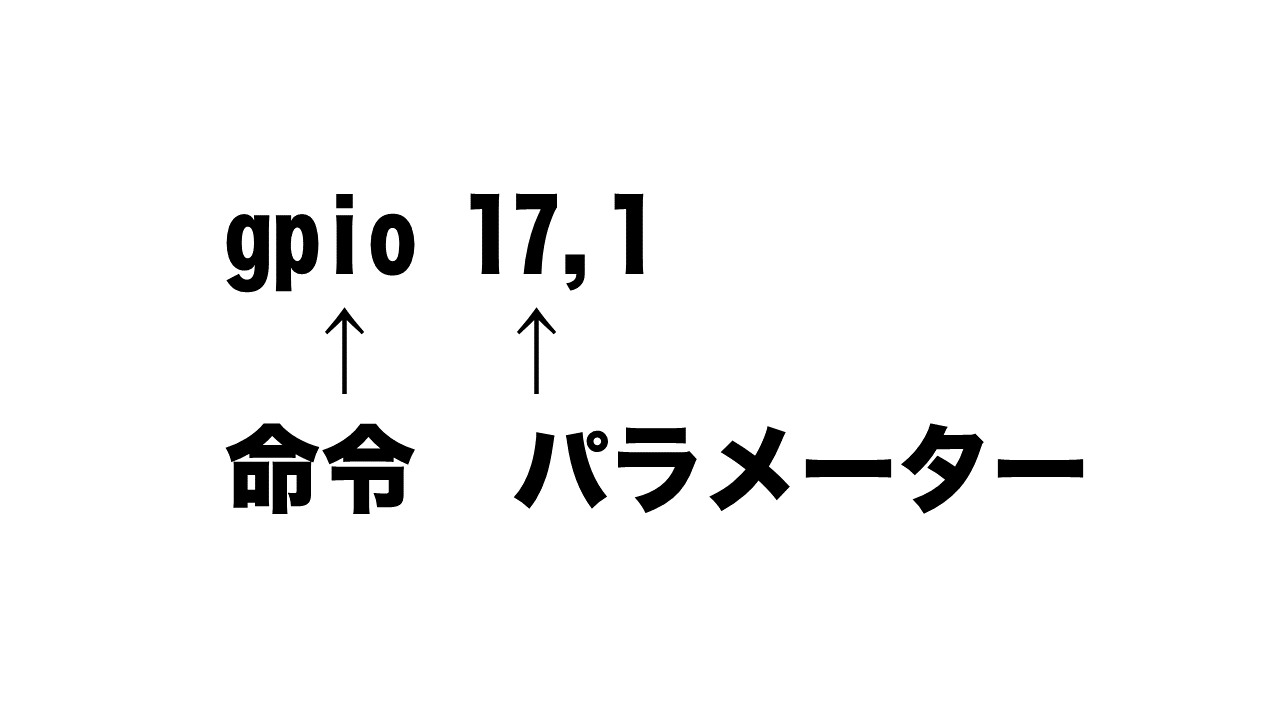
\includegraphics[keepaspectratio,width=8.017cm,height=4.512cm]{text02-img/text02-img024.png}}
\end{minipage}

\bigskip
\bigskip
\bigskip

たとえば、「gpio 17,1」という行を見てみましょう。

\bigskip

\ \ (HSPのルール)


\bigskip

\ \ 「gpio」はパソコンに指示を与える「命令」にあたります。

\ \ 「命令」の後に、細かい指示の内容を書きます。(パラメーターと呼ぶ)

\ \ 「命令」と「パラメーター」の間にはスペース(空白)を入れる


\bigskip

つまり、「gpio」が命令、「17」と「1」がパラメーターです。

パラメーターは、「,」によって複数書くことができます。

この「命令」は、コンピューターに何をさせるか、どんな機能を使うかを示しています。

ここで使っている「gpio」は、Raspberry PiのGPIOという端子をせいぎょします。


\bigskip

GPIOは、RaspberryPiの基板からせいぎょすることのできるスイッチのようなものです。

皆さんが使っているセンサーボードの上にあるスイッチやLEDは、GPIOとつながっていて、ON/OFFしたり、スイッチの状態を調べることができます。


\bigskip
\bigskip

\begin{minipage}{9.781cm}
\centering
{\upshape
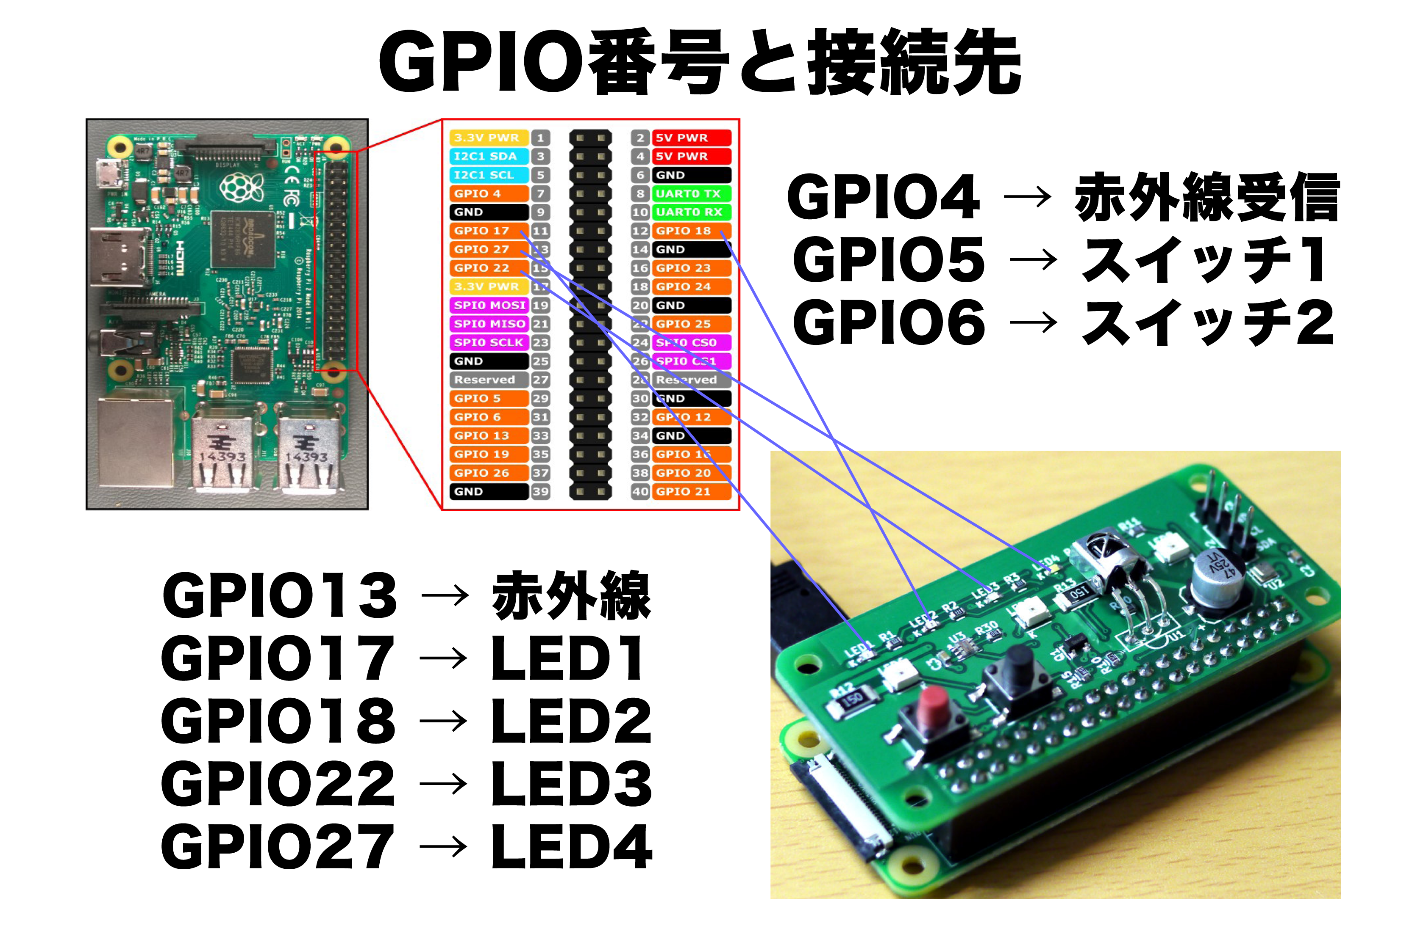
\includegraphics[keepaspectratio,width=12.409cm,height=7.62cm]{text02-img/text02-img025.png}}
\end{minipage}

\bigskip
\bigskip
\bigskip

gpioという命令によってLEDのON/OFFがせいぎょできるのかな…と何となく想像できますか?

GPIO
のONとOFFのスイッチを切り替えると、センサーボード上のLEDもON/OFFするということになります。


\bigskip

\ \ (HSPのルール)


\bigskip

\ \ gpio命令は、Raspberry PiのGPIOをせいぎょするための命令

\ \ gpioの後にスペースに続けて「IO番号」「,(カンマ)」「ON(1)/OFF(0)の値」を書く


\bigskip

\bigskip

つまり、「gpio 17,1」という命令は、「GPIO17をONにする」つまりLED1を点灯させることができます。
基板には、LED1〜4までのLEDがとうさいされているので、GPIO17,18,22,27をそれぞれ自由にON/OFFの状態にできるわけです。(赤外線やスイッチについては、また後で説明します。)


\bigskip

スクリプトエディタで、スクリプトを直接修正してみます。

スクリプトの中で「gpio 17,1」と書いてある行を探してから、ためしに下のように他の番号を入れてみましょう。


\bigskip

\ \ gpio 18,1


\bigskip


\bigskip

キーボードの入力や、修正のしかたがわからない人は、TAや周りの先生に聞いてみましょう。


\bigskip

修正したら[F5]を押してちゃんと動くか見てみましょう。

おや…LEDが点きっぱなしになりましたね。

実は、LEDがてんめつするためには、ONとOFFの2つを書きます。

つまり、「gpio 17,0」と書かれている部分も修正しなければなりません。


\bigskip

\ \ gpio 18,0


\bigskip

に修正して、もう一度[F5]を押しててんめつするか確認(かくにん)してみましょう。


\bigskip

\ \ (HSPのルール)


\bigskip

\ \ 1行目から順番に命令を実行してゆく。

\ \ 時間待ちをしたり、くり返したりすることができる。


\bigskip

wait命令は、一定時間停止するための命令です。

パラメーターの数字を修正すれば、てんめつの速度が変わります。

\bigskip
\bigskip

\begin{minipage}{9.781cm}
\centering
{\upshape
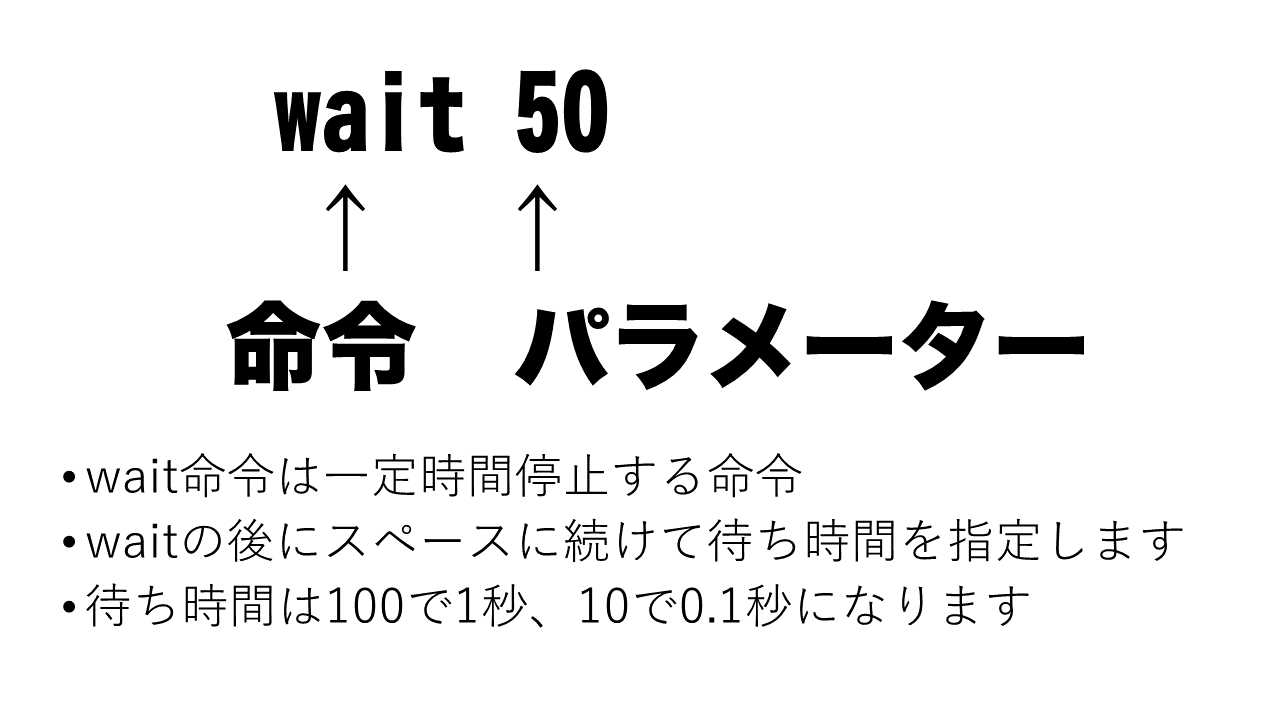
\includegraphics[keepaspectratio,width=10.372cm,height=5.837cm]{text02-img/text02-img026.png}}
\end{minipage}

\bigskip
\bigskip
\bigskip

このようにコンピューターにわかる言葉、スクリプトを正しく書くことで、その通りに動きます。

どんなに間違ったとしてもコンピューターがこわれることはありません。

うまく動かない時は、どうしてなのか考えてみて、わからない時は質問してみましょう。


\bigskip

\subsection{文字を表示する命令}
\bigskip
\bigskip

LEDがてんめつしている間、画面には「OK!」のメッセージが表示されています。

\bigskip
\bigskip

\begin{minipage}{9.781cm}
\centering
{\upshape
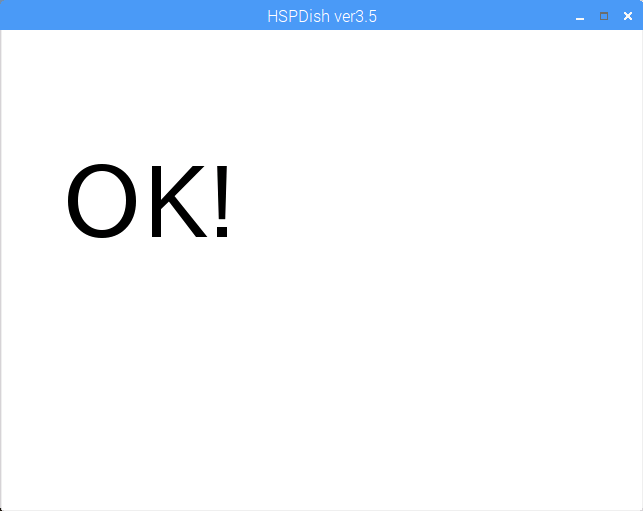
\includegraphics[keepaspectratio,width=5.741cm,height=4.572cm]{text02-img/text02-img027.png}
\flushleft

Figure \stepcounter{Figure}{\theFigure}: OK!のメッセージ}
\end{minipage}

\bigskip
\bigskip
\bigskip

実行されているスクリプトを見てみましょう。

「mes “OK!”」と書かれている行が関係ありそうですね。

ためしに{\textquotedbl}OK!{\textquotedbl}のかわりに自分の名前を入れてみましょう。


\bigskip

\ \ mes {\textquotedbl}takeda{\textquotedbl}


\bigskip

打ち込んだら[F5]を押してちゃんと動くか見てみましょう。


\bigskip

\ \ (HSPのルール)


\bigskip

\ \ mes命令は文字を画面に出す命令

\ \ mesの後にスペースに続けて表示したい文字を指定します

\ \ 必ず「{\textquotedbl}」で文字を囲むこと


\bigskip

mesという命令で文字を出すことができます。今度はパラメーターに「”」の記号で囲んだ文字を使っています。パラメーターで指定する時は、「”」で囲んだ文字か、数字になることを覚えておきましょう。


\bigskip

このようにコンピューターにわかる言葉、スクリプトを正しく書くことで、その通りに動いてくれます。

どんなに間違ったとしてもコンピューターがこわれることはありません。

HSPのルールを守らないとエラーが表示されてしまいます。

ターミナルの画面に、何行目でエラーが出たのかが表示されるので、その行を見直すといいでしょう。


\bigskip

\subsection{スクリプトの保存}
\bigskip
\bigskip

最後に自分で書き換えたスクリプトを保存する方法を忘れずに覚えておきましょう。

スクリプトをファイルとして保存しておけば、いつでも開いて続きから始めることができます。ファイル→「名前を付けて保存…」から、「mygpio.hsp」など自分の好きな名前で保存しておいてください。

\bigskip
\bigskip

\begin{minipage}{9.781cm}
\centering
{\upshape
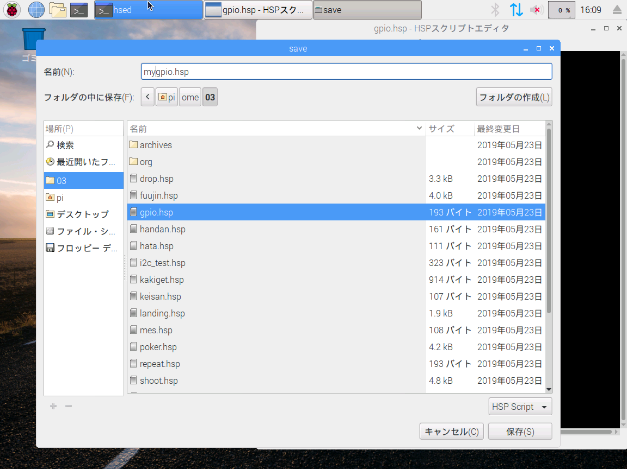
\includegraphics[keepaspectratio,width=6.976cm,height=4.944cm]{text02-img/text02-img028.png}
\flushleft

Figure \stepcounter{Figure}{\theFigure}: スクリプト保存のダイアログ}
\end{minipage}

\bigskip
\bigskip
\bigskip

\bigskip

\subsection{例題に挑戦しよう}

\bigskip
\bigskip

ここまで終わってしまった人は、以下の例題にも挑戦してみよう。


\bigskip

・命令のヘルプと検索のしかたを覚える

・文字に色をつけてみる(color命令)

・文字の位置やサイズを変えてみる(pos,font命令)

・四角形を描く命令を使ってみる(boxf命令)


\bigskip

例題の考え方がわからない時は、近くのTAか先生に聞いてください。

わからない所は、そのままにせず、必ず答えを見つけてから先に進みましょう。

\bigskip


\clearpage
\subsection{例題5 命令のヘルプと検索のしかたを覚える}
\bigskip
\bigskip

{\bfseries
考え方}

\bigskip

HSPで使うことのできる命令を調べたり、説明を読むための方法を覚えておきましょう。

HSPで書ける命令は、色々な種類があります。HSPスクリプトエディタで調べたい命令にカーソルを合わせて[F1]キーを押すことでヘルプが表示されます。

\bigskip

左上の入力枠に命令を入れて検索をすることができます。

試しに、「mes」「wait」などの命令を調べてみましょう。

\bigskip

\bigskip

{\bfseries
例題5 答え}


\bigskip

mes命令のヘルプが正しく表示されたかどうか確認(かくにん)してみましょう。

このページでは、HSPの命令やサンプル、関連命令などを検索することができます。

\bigskip
\bigskip

\begin{minipage}{9.781cm}
\centering
{\upshape
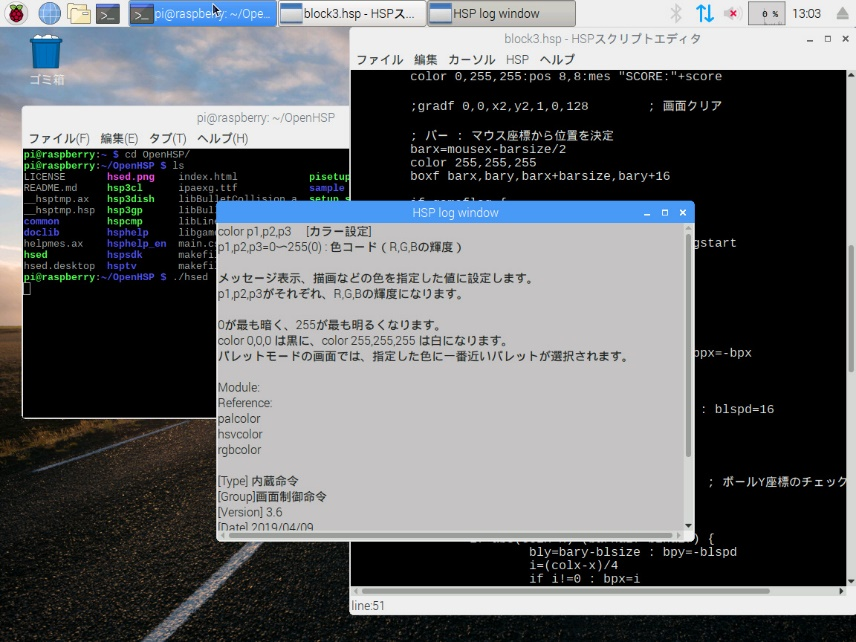
\includegraphics[keepaspectratio,width=9.895cm,height=7.421cm]{text02-img/text02-img029.jpg}
\flushleft

Figure \stepcounter{Figure}{\theFigure}: ヘルプの画面}
\end{minipage}

\bigskip
\bigskip
\bigskip



\clearpage
\subsection{例題6 文字に色を付けてみる}
\bigskip
\bigskip

{\bfseries
考え方}

\bigskip

mes命令で表示する文字に色を付けるにはcolor命令を使います。

\bigskip
\bigskip

\begin{minipage}{9.781cm}
\centering
{\upshape
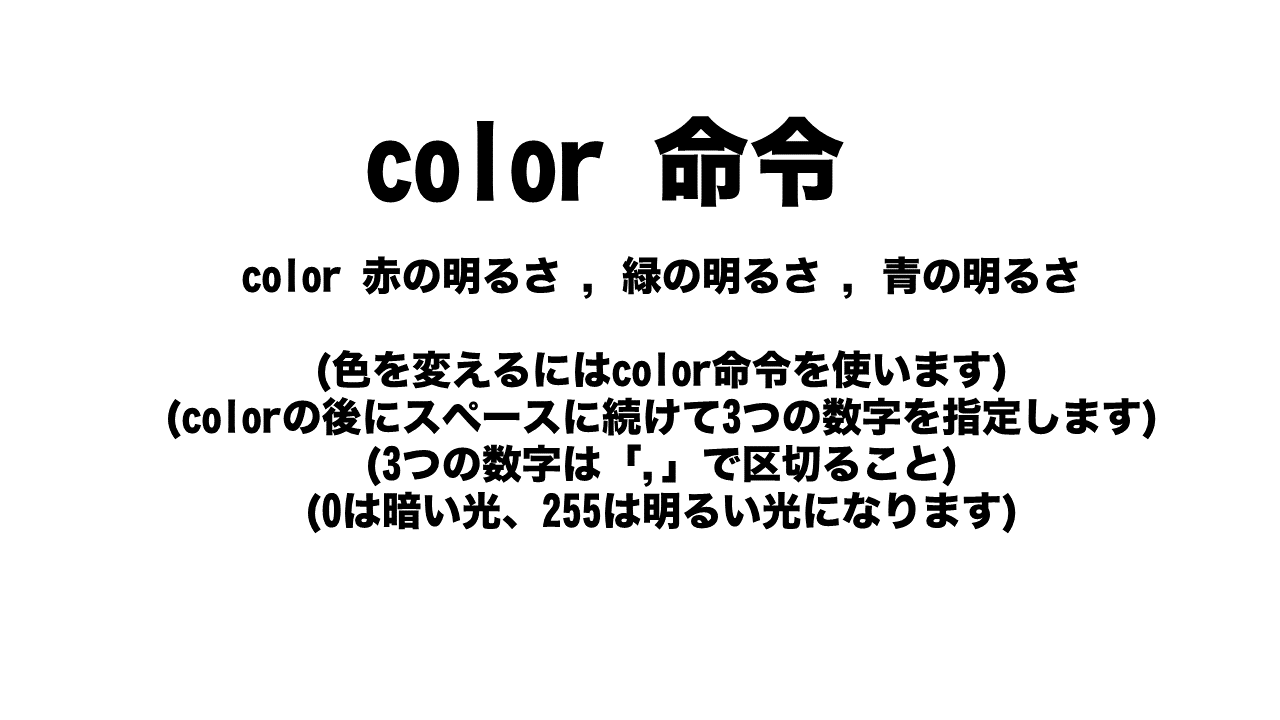
\includegraphics[keepaspectratio,width=12.277cm,height=5.08cm]{text02-img/text02-img030.png}}
\end{minipage}

\bigskip
\bigskip
\bigskip

明るさとは、その成分がどのくらい明るいかということを示している数値です。

明るさは、0がもっとも
暗くて、255が最も明るい状態になります。

これらを組み合わせて、1670万以上の色を
出すことができます。この時に指定する色のことをRGBと呼んでいます。

\bigskip
\bigskip

{\bfseries
RGBとは}

光の3原色は赤、緑、青紫ですが、赤と緑をまぜるとイエローに、緑と青紫をまぜるとシアンに、青紫と赤をまぜるとマゼンタになります。
光の3原色を等分にまぜると明るくなって、白色光になります。これを「加法混色(かほうこんしょく)」といいます。
RGBカラーはカラーテレビやモニタなどの「光り」で色を表現する方式です。

\bigskip
\bigskip

\begin{minipage}{9.781cm}
\centering
{\upshape
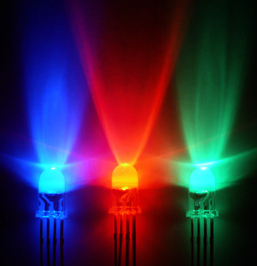
\includegraphics[keepaspectratio,width=3.854cm,height=3.988cm]{text02-img/text02-img033.jpg}}
\end{minipage}

\bigskip
\bigskip
\bigskip

RGBの意味は R:レッド(赤) G:グリーン(緑) B:ブルー(青)の頭文字です。
赤・緑・青それぞれの光の強さを0から255までの数値で表わします。
黒は、赤・緑・青のどれも光らせない(強さ0)ことで表現します。
白は赤・緑・青すべてを光らせた時(強さ255)の色になります。

モニターで色がついているのも、すべての点で3つの色(RGB)が光っているからです。コンピューターが、それぞれの点(ドット)をせいぎょして光らせているのです。


\bigskip
\bigskip

\begin{minipage}{11.781cm}
\centering
{\upshape
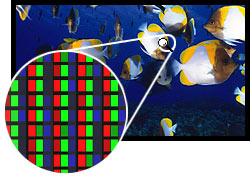
\includegraphics[keepaspectratio,width=3.854cm,height=3.988cm]{text02-img/text02-img034.jpg}
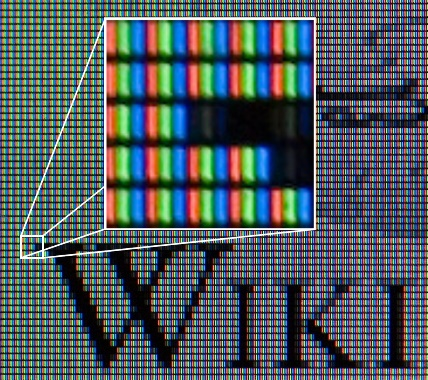
\includegraphics[keepaspectratio,width=3.854cm,height=3.988cm]{text02-img/text02-img035.jpg}}
\end{minipage}

\bigskip
\bigskip
\bigskip

mes命令の前に書かれているcolor命令の数字を変更することで、「OK!」の文字に使われている色を変えることができます。

自分で色を選んで、好きな色で文字を出してみましょう。

\bigskip


\bigskip

{\bfseries
例題6 答え}


\bigskip

必ず、mes命令が実行されるよりも前(上の行)にcolor命令を書きます。

代表的な色は次のようになります。参考にして思った通りの色になっているか確認(かくにん)してみましょう。

\bigskip

\ \ \ \ color 0 ,0 ,0 ; ← 黒 

\ \ \ \ color 0 ,0 ,255 ; ← 青 

\ \ \ \ color 255 ,0 ,0 ; ← 赤 

\ \ \ \ color 255 ,0 ,255 ; ← 紫 

\ \ \ \ color 0 ,255 ,0 ; ← 緑 

\ \ \ \ color 0 ,255 ,255 ; ← 水色 

\ \ \ \ color 255 ,255 ,0 ; ← 黄色 

\ \ \ \ color 255 ,255 ,255 ; ← 白 


\bigskip
\bigskip

「; ← 黒」のように行の中で「;」が入っている部分から先は「コメント」として扱われます。

「;」から先は、命令を書いても実行の時にも無視されます。

「コメント」は、その行でやっていること、残しておきたいメモなどを書くことのできる機能です。

\bigskip
\bigskip



\clearpage
\subsection{例題7 文字のサイズを変えてみる}
\bigskip
\bigskip

{\bfseries
考え方}

\bigskip

mes命令で表示する文字のサイズを変えるにはfont命令を使います。


\bigskip

\ \ (例)

\ \ font “”,100


\bigskip

font命令の後にスペースに続けて「””」、さらに「,」と大きさが書かれています。

たとえば、この「100」をもっと大きな数字にしてみて、文字が大きくなるのを確認(かくにん)しましょう。

\bigskip

\bigskip

{\bfseries
例題7 答え}

\bigskip

必ず、mes命令が実行されるよりも前(上の行)にfont命令を書きます。

font命令で指定するパラメーターのは文字のサイズで大きい数になるほど文字も大きくなります。

逆に小さな数にすることで、小さな文字になります。


\bigskip

\ \ (HSPのルール)


\bigskip

\ \ font命令はフォントの形と大きさを決めるための命令

\ \ 「“”,70」、の70はそのサイズ


\bigskip

実際に試してみて、文字のサイズが変わったらTAや周りの友達にも見せてあげましょう。


\clearpage
\subsection{例題8 文字の表示位置を変えてみる}
\bigskip
\bigskip

{\bfseries
考え方}

\bigskip

mes命令で表示する文字の表示位置を変えるにはpos命令を使います。


\bigskip

\ \ (例)

\ \ pos 160,200


\bigskip

パラメーターの数字2つを、増やしたり減らしたりしながら、文字の位置がどのように変わるか試してみましょう。

\bigskip

\bigskip

{\bfseries
例題8 答え}

\bigskip

必ず、mes命令が実行されるよりも前(上の行)にpos命令を書きます。


\bigskip

\ \ (例)

\ \ pos 160,200


\bigskip

「160」の部分が左からの位置。

「200」の部分が上からの位置になります。

位置を指定するためには、たてよこの2つ数字が必要です。

「横(よこ)の位置」「縦(たて)の位置」は、左上からの点(ドット)の数なので覚えておきましょう。


\bigskip

\ \ (HSPのルール)


\bigskip

\ \ 文字を出す位置を変えるにはpos命令を使います

\ \ posの後はスペースに続けて2つの数字を指定します

\ \ 2つの数字は「,」で区切ること

\ \ 2つの数字は「横(よこ)の位置」「縦(たて)の位置」を指定する


\bigskip

実際に試してみて、文字の表示位置が変わったらTAや周りの友達にも見せてあげましょう。



\clearpage
\subsection{例題9 四角形を描いてみる}
\bigskip
\bigskip

{\bfseries
考え方}

\bigskip

四角形を描く命令、boxf命令を使ってみましょう。

まず簡単に背景の色を変えてみましょう。

\ \ color 255,255,255

\ \ boxf

これで白い背景になります。

\bigskip
\bigskip

\begin{minipage}{9.781cm}
\centering
{\upshape
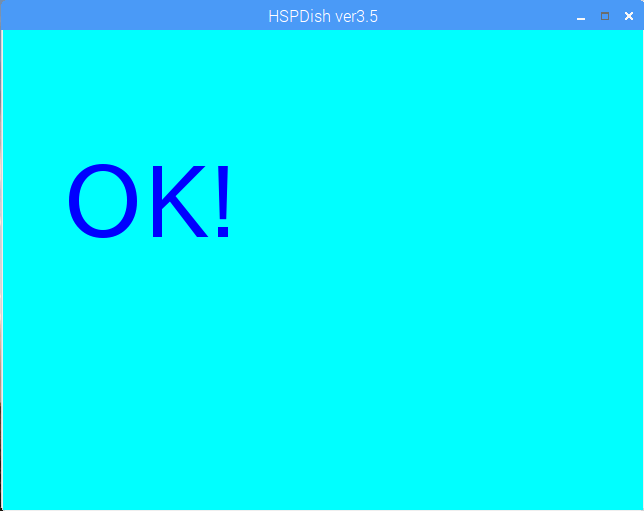
\includegraphics[keepaspectratio,width=6.006cm,height=4.77cm]{text02-img/text02-img036.png}}
\end{minipage}

\bigskip
\bigskip
\bigskip

\ \ color 255,0,255

\ \ boxf

\bigskip

のように修正すると色が変わります。

文字と同じようにcolor命令で四角形の色を変えることができます。

\bigskip

\ \ (例)

\ \ boxf 100,200,200,250


\bigskip

パラメーターの数字4つを、増やしたり減らしたりしながら、四角形がどのように変わるか試してみましょう。


\bigskip


\bigskip

{\bfseries
例題9 答え}

\bigskip

boxf命令は4つのパラメーターを指定します。


\bigskip

\ \ (HSPのルール)


\bigskip

\ \ 四角形を描くにはboxf命令を使います

\ \ boxfの後はスペースに続けて4つの数字を指定します

\ \ 4つの数字は「,」で区切ること

\ \ 4つの数字は「左上横(よこ)の位置」「左上縦(たて)の位置」「右下横(よこ)の位置」「右下縦(たて)の位置」を指定する

\ \ 4つのパラメーターを省略(しょうりゃく)すると全画面を塗りつぶします


\bigskip

実際に試してみて、四角形が描けたらTAや周りの友達にも見せてあげましょう。



  % Modify:

\clearpage
\section{ゲームを改造してみよう}
\subsection{ドロップパズルの改造}
\bigskip
\bigskip

ファイル→「開く」メニューから/home/ユーザー名/02のフォルダに移動してから、「drop.hsp」を読み込んでみましょう。

\bigskip
\bigskip

\begin{minipage}{9.781cm}
\centering
{\upshape
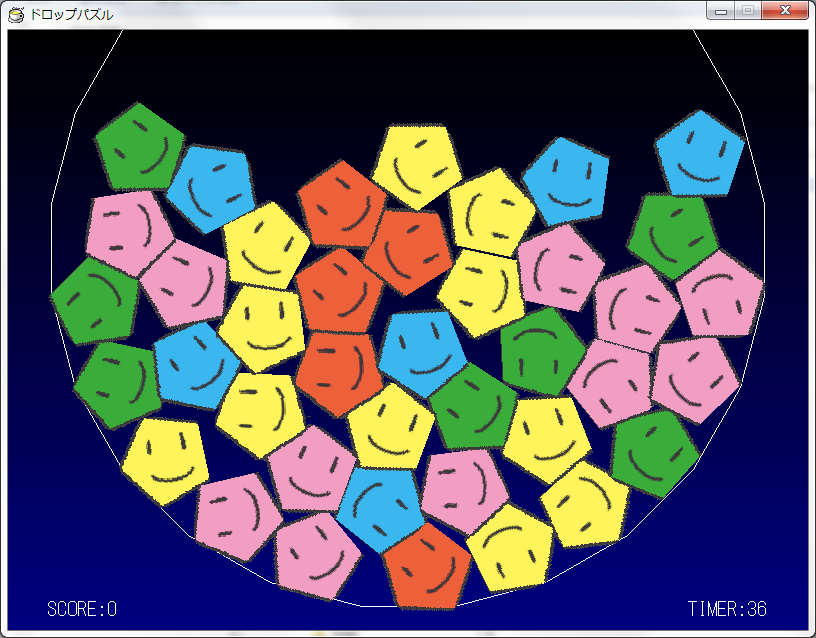
\includegraphics[keepaspectratio,width=8.356cm,height=6.544cm]{text02-img/text02-img015.png}
\flushleft

Figure \stepcounter{Figure}{\theFigure}: ドロップパズルゲームの画面}
\end{minipage}

\bigskip
\bigskip
\bigskip

ドロップパズルゲームを改造して、自分だけのゲームに変えてみます。

スクリプトは、簡単に修正できることを学びました。実は、ゲームの中の絵も自由に修正することができます。

\bigskip
\bigskip

\subsection{GIMPを使ってみよう}
\bigskip
\bigskip

ここでは、第1回で使ったRaspberry Piで絵を描くためのプログラム「GIMP」を使ってみます。

ファイルマネージャーの画面から、「/home/ユーザー名/02」フォルダにある「koma.png」のアイコンで右クリックを押して、「GIMP ( GNU Image Manipulation Program )」のメニューを選ぶすることでツールを起動させることができます。

これで、「koma.png」を読み込んで下絵とすることができます。

\bigskip
\bigskip

\begin{minipage}{9.781cm}
\centering
{\upshape
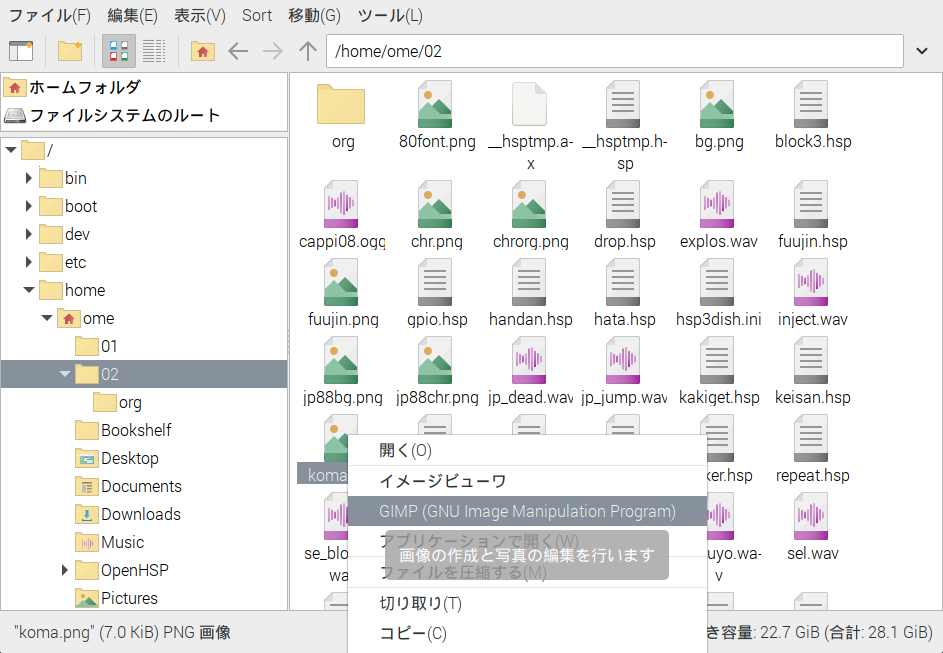
\includegraphics[keepaspectratio,width=10.583cm,height=7.938cm]{text02-img/s_komapng.png}
\flushleft

Figure \stepcounter{Figure}{\theFigure}: koma.pngからGIMPを起動するところ}
\end{minipage}

\bigskip
\bigskip
\bigskip



\subsection{ドロップパズルの中身を変えてみよう}
\bigskip
\bigskip

GIMPを使って、ドロップパズルのゲームで使われた絵を改造してみましょう。

GIMPは、絵のデータを読み込んで、自分で好きに変更することができます。

変更した絵は、ふたたび保存することができます。

\bigskip
\bigskip

\begin{minipage}{9.781cm}
\centering
{\upshape
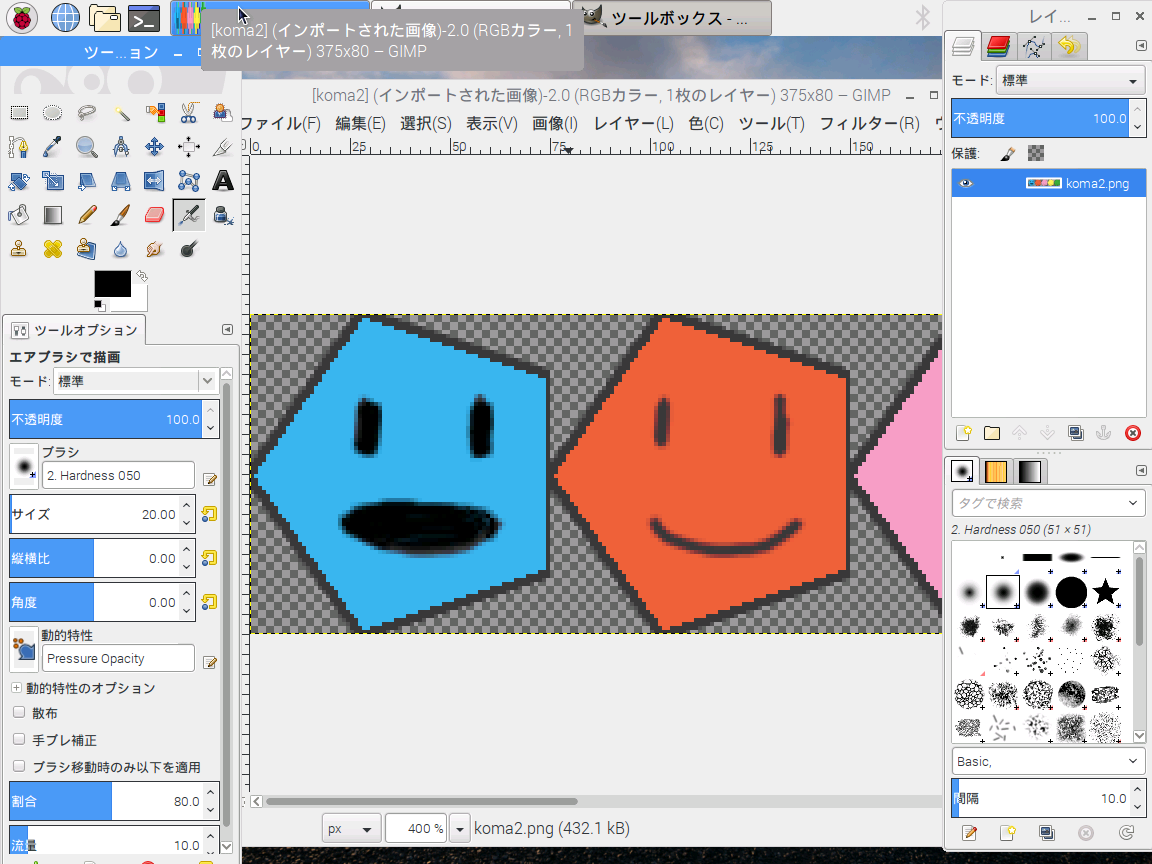
\includegraphics[keepaspectratio,width=10.403cm,height=7.811cm]{text02-img/text02-img038.png}
\flushleft

Figure \stepcounter{Figure}{\theFigure}: koma.pngを修正している画面}
\end{minipage}

\bigskip
\bigskip
\bigskip

このキャラクターを別な絵に書き換えればゲームの絵も変わります。
パレットで色を選んで、鉛筆のツールで絵を書いていきます。
元の絵があった部分を書き換えて他の絵柄にしてみましょう。

\bigskip
\bigskip

\begin{minipage}{9.781cm}
\centering
{\upshape
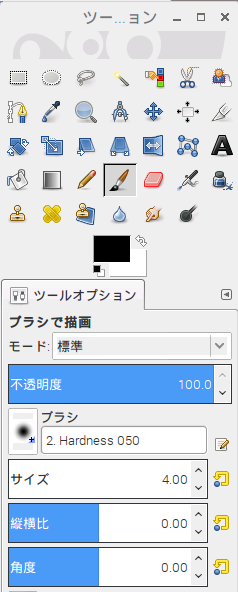
\includegraphics[keepaspectratio,width=4.075cm,height=10.16cm]{text02-img/text02-img039.png}
\flushleft

Figure \stepcounter{Figure}{\theFigure}: ツールのウインドウ}
\end{minipage}

\bigskip
\bigskip
\bigskip

画像が小さい場合は、画像の下にある「100\%」の右側にあるボタンを押して、「400\%」「800\%」などを選ぶと拡大されます。

絵を修正する時には、ツールアイコンの中から「ブラシ」を選択して、サイズを4〜6くらいの数字に変えてから絵の上で、マウスボタンを押しながら動かして色を置きます。


\bigskip

色を変更する場合は、ツールパレットの描画色をクリックして、「描画色の変更」ダイアログを出してから好きな色を選びます。

\bigskip
\bigskip

\begin{minipage}{9.781cm}
\centering
{\upshape
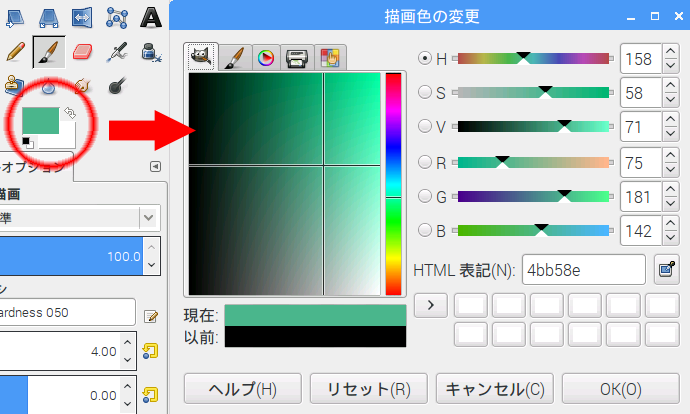
\includegraphics[keepaspectratio,width=10.993cm,height=6.588cm]{text02-img/text02-img040.png}
\flushleft

Figure \stepcounter{Figure}{\theFigure}: 色をえらぶところ}
\end{minipage}

\bigskip
\bigskip
\bigskip

元の絵を書き換えたら、ファイル→「koma.pngに上書きエクスポート」を選んで保存します。

作業が終わったら、最後にファイル→「終了」を選んでGIMPアプリケーションを閉じるのを忘れないでください。

通常の「保存」メニューを選択すると元のPNGファイルではなく、GIMP専用のファイル形式でて保存されてしまいます。

今回は、PNGファイルだけを保存したいので、「koma.pngに上書きエクスポート」を選んで保存するようにしてください。

\bigskip

変更した画像でゲームを動かしてみましょう。

HSPスクリプトエディタを起動して、「drop.hsp」を読み込みます。

\ [F5]キーを押して実行して変わっていれば成功です。


\bigskip

本当にスクリプトからゲームが作られているのか確かめてみましょう。

たとえば、ドロップパズルゲームのスクリプトには、「name=”ドロップパズル”」と書かれている部分があります。

\bigskip
\bigskip

\begin{minipage}{9.781cm}
\centering
{\upshape
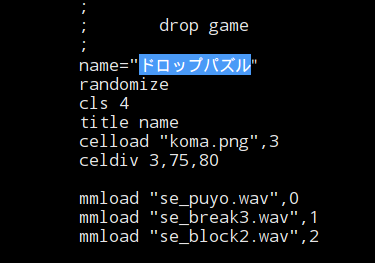
\includegraphics[keepaspectratio,width=9.049cm,height=6.346cm]{text02-img/text02-img014.png}
\flushleft

Figure \stepcounter{Figure}{\theFigure}: ドロップパズルのスクリプト}
\end{minipage}

\bigskip
\bigskip
\bigskip

これを、「name=”ドロドロパズル”」など他の文字に変えてみてください。

[F5]キーで実行して、どこが変わっているか確認(かくにん)してみましょう。

\bigskip

「k=rnd(5)」という部分を探してみましょう。

これは106行目にあります。カーソルがある行の数は左下に「line:〇〇〇」表示されていますので確認(かくにん)してみましょう )

この「5」を「3」などもっと少ない数に変えてみるとどうなるか確認(かくにん)してみましょう。

\bigskip
\bigskip

\begin{minipage}{9.781cm}
\centering
{\upshape
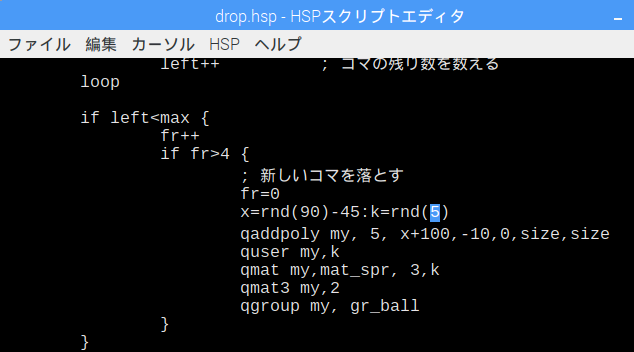
\includegraphics[keepaspectratio,width=12.753cm,height=7.064cm]{text02-img/text02-img041.png}}
\end{minipage}

\bigskip
\bigskip
\bigskip

変更したスクリプトは、ファイル→「上書き保存」によりdrop.hspに保存することができます。

別な名前で保存したい時には、ファイル→「名前を付けて保存…」で新しいファイルとして保存することができます。

これから先、さらに色々な部分を変えてみながら、プログラムの動きについて覚えていきましょう。


\bigskip

これで、あなたが改造したオリジナルのパズルゲームになりました。

\bigskip



\subsection{例題に挑戦しよう}

\bigskip
\bigskip

ここまで終わってしまった人は、以下の例題にも挑戦してみよう。


\bigskip

・シューティングゲーム(shoot)の絵を改造する

・シューティングゲーム(shoot)のスクリプトを改造する

・タイトルを変えてみよう

・敵や味方の強さを変えてみよう

・ゲーム全体の速さを変えてみよう

\bigskip

例題の考え方がわからない時は、近くのTAか先生に聞いてください。

わからない所は、そのままにせず、必ず答えを見つけてから先に進みましょう。

\bigskip


\clearpage
\subsection{例題10 シューティングゲームの絵を改造する}
\bigskip
\bigskip

{\bfseries
考え方}

\bigskip

シューティングゲーム(shoot.hsp)の絵を改造して自分だけの絵にしてみましょう。

シューティングゲームの絵は、「/home/ユーザー名/02/chr.png」というファイルに保存されています。

改造ができたらTAや周りの友達にも見せてあげましょう。

\bigskip

\bigskip

{\bfseries
例題10 答え}


\bigskip

教科書でドロップパズルの絵を修正したのと同じように、GIMPを使ってシューティングゲームの絵を修正します。


\bigskip

ファイルマネージャーの画面から、「/home/ユーザー名/02」フォルダにある「chr.png」のアイコンで右クリックを押して、「GIMP ( GNU Image Manipulation Program )」のメニューを選ぶすることでツールを起動させることができます。

これで、「chr.png」を読み込んで下絵とすることができます。

\bigskip
\bigskip

\begin{minipage}{9.781cm}
\centering
{\upshape
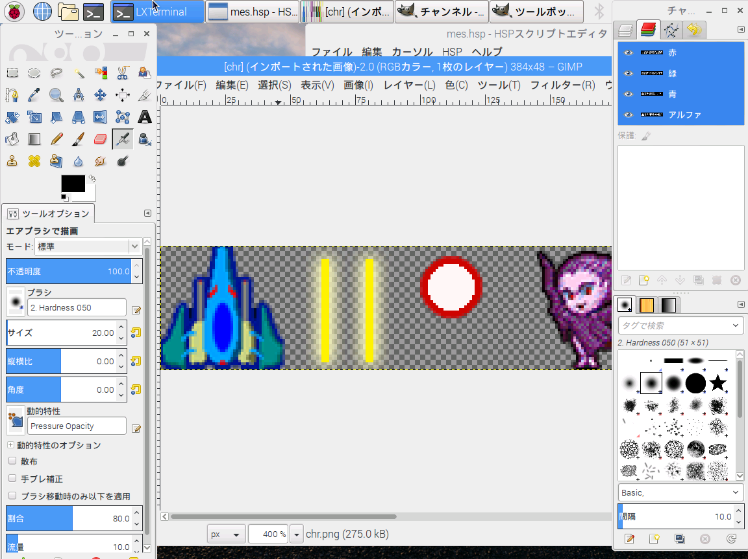
\includegraphics[keepaspectratio,width=8.625cm,height=6.459cm]{text02-img/text02-img042.png}
\flushleft

Figure \stepcounter{Figure}{\theFigure}: chr.pngを読み込んだ画面}
\end{minipage}

\bigskip
\bigskip
\bigskip

左にあるのが自機、その右にあるのがレーザー、その右は敵の弾です。ゲームのキャラクターを改造してみましょう。

作業が終わったら、ファイル→「chr.pngに上書きエクスポート」を選んで保存します。


\bigskip

時間のある人は、他の絵の書き換えにも挑戦してみましょう。

背景は「bg.png」、キャラクターは「chr.png」、タイトルは「title.png」です。

\bigskip

※もし、chr.png の内容を元に戻したい時には、/usr/local/share/ome/02/chr.png のファイルを /home/ユーザー名/02 フォルダに上書きでコピーすれば元に戻せます。

\bigskip

GIMPを使い終わったら、最後にファイル→「終了」を選んでGIMPアプリケーションを閉じてください。


\clearpage
\subsection{例題11 シューティングゲームの内容を改造する}
\bigskip
\bigskip

{\bfseries
考え方}

\bigskip

シューティングゲーム(shoot.hsp)のスクリプトを改造してゲームの内容を変えてみましょう。

シューティングゲームのスクリプトは、「/home/ユーザー名/02/shoot.png」というファイルに保存されています。

\bigskip

\bigskip

まず、HSPスクリプトエディタを起動して、ファイル→「開く」メニューから「shoot.hsp」を読み込んでください。

\bigskip
\bigskip

\begin{minipage}{9.781cm}
\centering
{\upshape
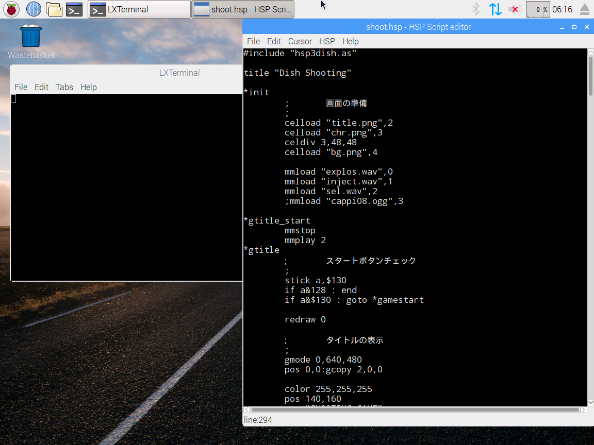
\includegraphics[keepaspectratio,width=6.853cm,height=5.135cm]{text02-img/text02-img043.png}
\flushleft

Figure \stepcounter{Figure}{\theFigure}: shoot.hspを読み込んだところ}
\end{minipage}

\bigskip
\bigskip
\bigskip

でたらめに書き直してもエラーが出るだけです。

タイトルに表示されている文字、色、場所はパラメーターを変えられます。

命令にあたる部分は変えないようにしましょう。


\bigskip

・プレイヤーのミサイル連射を増やしてみる


\bigskip

\ \ (「lmax=4」が連射の数です)

\ \ 敵の数を変えてみる

\ \ (「einter=18」が出てくる確率「emax=16」が最大の数です)

\ \ 敵の弾数を変えてみる

\ \ \ \ (「msrint=2」の2を大きくすると増えます「amax=16」は最大の数です)

\ \ ゲームの速度を変えてみる

\ \ (「await
18」という部分の18を少ない数にしてみましょう)

\bigskip
\bigskip

{\bfseries
例題11 答え}


\bigskip

ゲームを改造することで、難しくなったり、簡単になったりします。

改造ができたらTAや周りの友達にも見せてあげましょう。


\bigskip

※プログラムをあまり改造しすぎると、動かなくなったり、パソコンの動きが遅くなってしまうことがあります。その時は、先生に聞くか、「/usr/local/share/ome/02/」フォルダ内の元のファイル(shoot.hsp)をもう一度コピーして使ってみてください。



  % Program:

\clearpage
\section{プログラムの仕組みを知ろう}
\subsection{プログラムの流れをあやつろう}
\bigskip
\bigskip

スクリプトに旗を立てる方法を覚えましょう。旗というのは屋上についてヒラヒラしたり山の頂上に立ってるものです。スクリプトの旗は目印になる場所を意味します。自分で好きな名前をつけてスクリプトの中に目印として旗を立てておくことができます。

ファイル→「開く」メニューから「hata.hsp」を読み込みましょう。


\bigskip

*hata

\ \ redraw 0

\ \ pos 0,0

\ \ mes {\textquotedbl}えっさ{\textquotedbl}

\ \ redraw 1

\ \ wait 50

\ \ redraw 0

\ \ pos 0,0

\ \ mes {\textquotedbl}   ほいさ{\textquotedbl}

\ \ redraw 1

\ \ wait 50

\ \ goto *hata


\bigskip

[F5]キーを押して実行すると、「えっさ」と「ほいさ」の文字が交互に表示されます。

スクリプトの行数は少ないのに、何度もくり返して実行されているのはなぜでしょう。

これが、旗の機能を使った例です。

旗のことをHSPではラベルと呼んでいます。


\bigskip

\ \ (HSPのルール)


\bigskip

\ \ 旗は「*」の後に旗の名前を自由に決めて書くことができる

\ \ (ただし命令と同じ名前は使えません)

\ \ goto命令は指定したラベル(旗)に飛ぶための命令

\ \ gotoの後にスペースに続けて飛び先のラベル(旗)を指定します

\ \ goto命令が実行された後は飛び先のラベル(旗)から実行が続けられます


\bigskip

つまり、1行目からスクリプトが実行されていますが、「goto
*hata」まで来ると、また「*hata」の行まで戻ってしまいます。こうして、このスクリプトは、「*hata」の行から「goto
*hata」までを永遠にくり返します。

このようにくり返しにより、大量の作業をこなしてしまうのがプログラムの凄いところです。

\bigskip

\ \ (HSPのルール)

\bigskip

\ \ 「redraw 0」から「redraw
1」は画面を更新するための命令

\ \ 画面を描き始める前に「redraw
0」を書いておく

画面を描き終わったら「redraw
1」を書いておく


\bigskip

自分なりに、mesのメッセージや、wait命令の待ち時間を変更して、どのような結果になるか試してみましょう。

\bigskip
\bigskip


\subsection{変数と計算}
\bigskip
\bigskip

プログラミングを覚える上で、とても重要な変数というものについて覚えていきましょう。

変数はどんなコンピューター言語でも使われている大切な機能です。

どんなものなのか、まずスクリプトを見てみましょう。

ファイル→「開く」メニューから「keisan.hsp」を読み込みましょう。


\bigskip

\ \ \ \ x=100

\ \ \ \ pos 20,120

\ \ \ \ color 0,0,255

\ \ \ \ mes {\textquotedbl}こたえは{\textquotedbl}+x


\bigskip

実行すると、画面の中央上に「こたえは100」が表示されましたね。

mes命令の”こたえは”の後ろに「+x」が付けられています。ここに出て来る「x」が「変数」です。

\bigskip
\bigskip

\begin{minipage}{9.781cm}
\centering
{\upshape
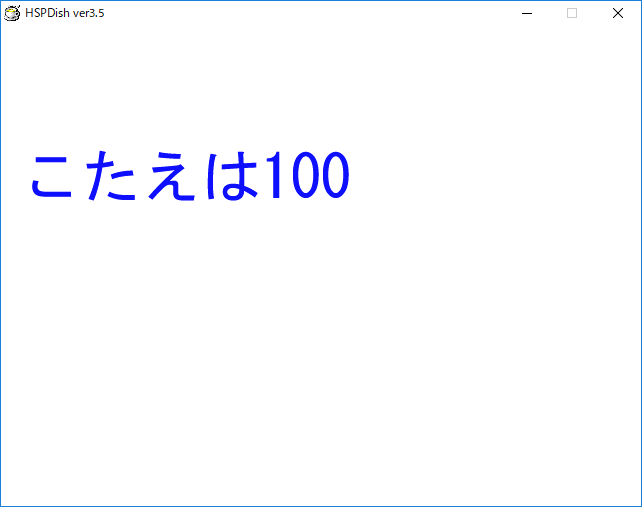
\includegraphics[keepaspectratio,width=7.382cm,height=5.831cm]{text02-img/text02-img044.png}
\flushleft

Figure \stepcounter{Figure}{\theFigure}: keisan.hspの実行画面}
\end{minipage}

\bigskip
\bigskip
\bigskip

変数はよく、「いれもの」にたとえられます。数値をきおくしておく、「いれもの」です。

「いれもの」には名前をつけることができます。たとえば「x」という名前の「いれもの」に数値を入れておくには、「x=100」のように書きます。

\bigskip
\bigskip

\begin{minipage}{9.781cm}
\centering
{\upshape
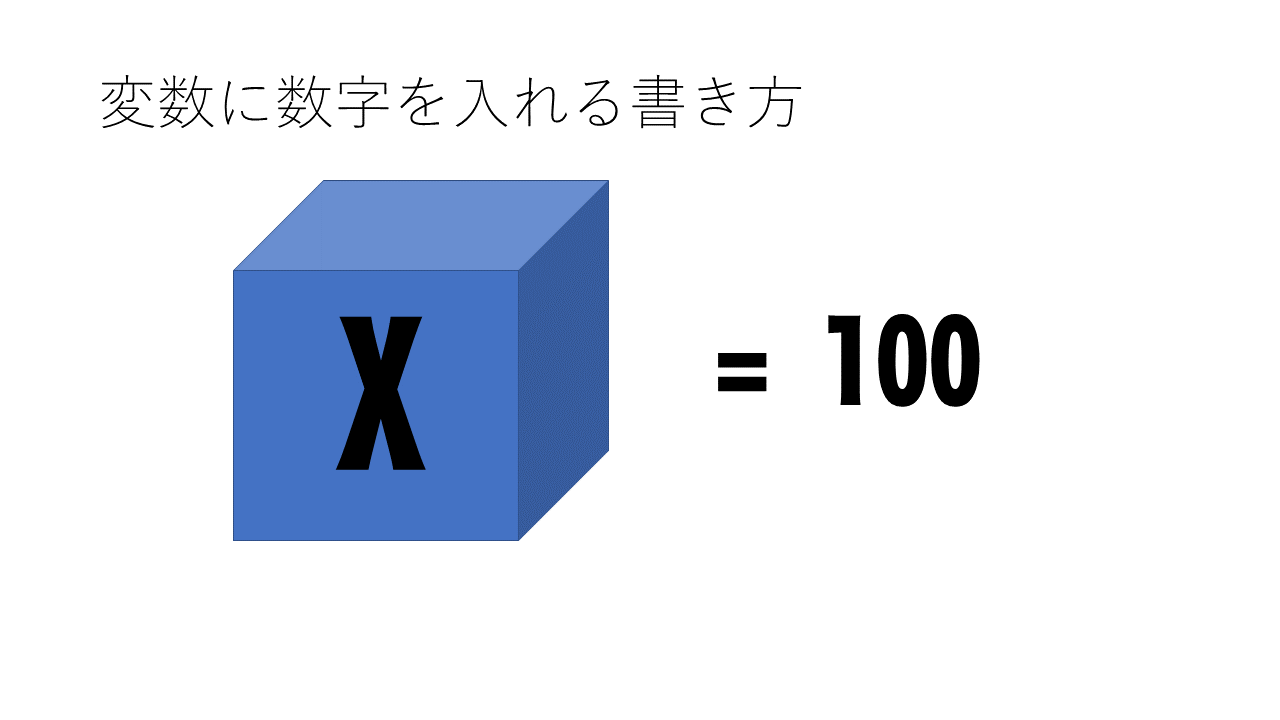
\includegraphics[keepaspectratio,width=10.478cm,height=5.106cm]{text02-img/text02-img045.png}}
\end{minipage}

\bigskip
\bigskip
\bigskip

このスクリプトではxという名前をつけてあります。これを変数xと呼びます。(名前は1文字でなく長い名前でもかまいません。日本語でもいいです。でも打ち込みやすいので1文字でもよく使われます)

名前は命令と同じものは使えないので注意しましょう。


\bigskip

「x=100」でxという名前の変数に100という数値が入ります。これを「代入」と呼んでいます。変数に数値を入れておくと命令で指定するパラメーターとして指定することができるようになります。

つまり「pos 100,120」を、「pos x,120」と書くこともできるのです。


\bigskip

\ \ (HSPのルール)


\bigskip

\ \ 「変数の名前=数値」で変数に値を入れることができる(代入)

\ \ 変数に数値を入れておくとパラメーターとして使える

\ \ mes命令の中で「+変数」を書くことで変数の中身を表示できる

\bigskip

変数に値を代入しておくことで同じ数値を指定する部分をまとめて変更したり、命令と別な場所で指定をすることができるようになります。

\bigskip

ほかにも、数値を書く部分に記号を入れて計算をすることができます。

計算は電卓などで使われている四則演算が基本になります。

\bigskip
\bigskip

\begin{minipage}{9.781cm}
\centering
{\upshape
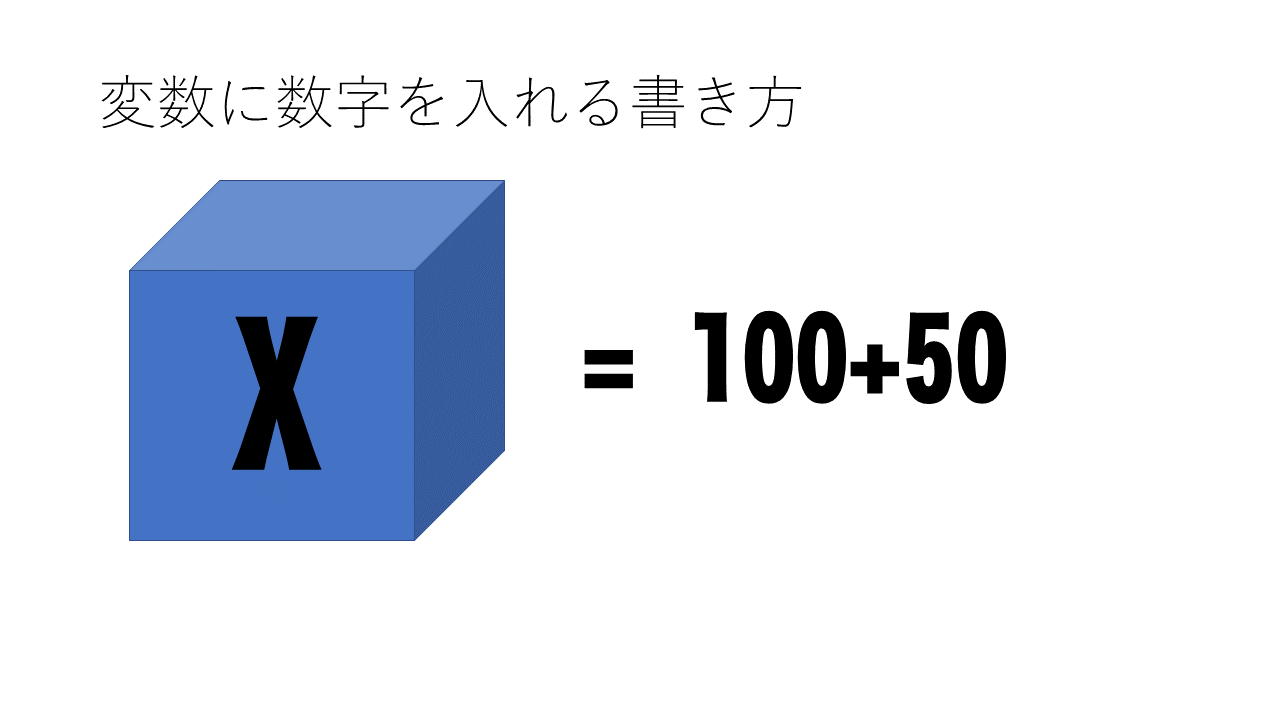
\includegraphics[keepaspectratio,width=11.695cm,height=5.741cm]{text02-img/text02-img046.png}}
\end{minipage}

\bigskip
\bigskip
\bigskip

\ \ (HSPのルール)


\bigskip

\ \ 数式とは、数値と変数、またはそれらを計算式でつなげて書くこと

\ \ 「+」は足し算、「-」は引き算
、「*」は掛け算(×)、「/」は割り算(÷) 


\bigskip

数式とはつまり、数値を指定する場所に1+1と書いたら2を書いたのと同じことになる、ということです。(コンピューターですから計算は大の得意です)

つまり、「x=100+20」は「x=120」と同じことになるのです。

変数と計算で何ができるのか、まだよくわからない人も多いと思いますが、あわてずにゆっくり覚えるようにしましょう。

\bigskip
\bigskip

\subsection{乱数を使ってみよう}
\bigskip
\bigskip

変数を使った例をもう1つ紹介します。ファイル→「開く」メニューから「stars.hsp」を読み込みましょう。100個の「☆」をmes命令で画面に表示しています。

ここでは、「☆」を表示する位置をバラバラにするために乱数を使用しています。

乱数は、ゲームなどでよく使われている要素の1つで、コンピューターが選んだバラバラな数字を作るものです。

バラバラな数字は、決められた数字の範囲で作ることができ、何が出るかは誰にも予想ができません。

\bigskip
\bigskip

\begin{minipage}{9.781cm}
\centering
{\upshape
\includegraphics[keepaspectratio,width=7.99cm,height=6.297cm]{text02-img/text02-img047.png}
\flushleft

Figure \stepcounter{Figure}{\theFigure}: stars.hspの実行画面}
\end{minipage}

\bigskip
\bigskip
\bigskip

スクリプトを見てみましょう。

\bigskip

\ \ \ \ repeat 100

\ \ \ \ x=rnd(640)

\ \ \ \ y=rnd(480)

\ \ \ \ pos x,y

\ \ \ \ mes {\textquotedbl}☆{\textquotedbl}

\ \ \ \ loop

\bigskip

変数xと変数yは、pos命令で「☆」を表示する位置をきおくするものとして使われています。

「x=rnd(640)」は、0〜639(640通り)までのバラバラな数字を変数xに代入します。このような書き方を「関数」と呼んでいます。

\bigskip
\bigskip

\begin{minipage}{9.781cm}
\centering
{\upshape
\includegraphics[keepaspectratio,width=11.906cm,height=5.662cm]{text02-img/text02-img048.png}}
\end{minipage}

\bigskip
\bigskip
\bigskip

\ \ (HSPのルール)


\bigskip

\ \ 「変数=rnd(乱数の最大値)」でバラバラな数字を得ることができる

\ \ 関数は、「変数=関数(パラメーター)」という書き方で使うことができる

\bigskip

「y=rnd(480)」も同様に0〜479までの数字を代入します。画面のサイズが、横(よこ)640、縦(たて)480ですから、画面上のでたらめな位置をpos命令で指定することができます。

repeat命令で100個の「☆」を描いていますが、この数字を変えたり(あまり大きな数字にすると遅くなるので注意してください)、乱数の範囲を変えてみながら、どのように画面が変化するか確認(かくにん)してみましょう。

余裕のある人は、でたらめな色で「☆」をたくさん表示する方法を考えてみてください。

\bigskip
\bigskip

\subsection{条件判断とは}
\bigskip
\bigskip

変数と数字を使って計算ができることはわかりました。さらにもう1つ、重要な要素として「条件判断」を覚えることができれば、プログラミングの大きな関門を1つ越えることになります。

それほど、「条件判断」はプログラミングの大きな要素であり、「条件判断」なしでは大きなプログラムを作ることはできません。

\bigskip
\bigskip

\begin{minipage}{9.781cm}
\centering
{\upshape
\includegraphics[keepaspectratio,width=12.33cm,height=6.939cm]{text02-img/text02-img049.png}}
\end{minipage}

\bigskip
\bigskip
\bigskip

\ \ (HSPのルール)


\bigskip

\ \ if命令により条件を判断することができる

\ \ ifの後にスペースに続けて条件式を指定します

\ \ その後で「:」に続けて条件が正しい時に実行される命令を書きます


\bigskip

\ \ (条件式はいくつか書き方があります)


\bigskip

\ \ \ \ 条件式 \ \ \ \ \ \ \ \ \ 意味

\ \ \ \ {}-{}-{}-{}-{}-{}-{}-{}-{}-{}-{}-{}-{}-{}-{}-{}-{}-{}-{}-{}-{}-{}-{}-{}-{}-{}-{}-{}-{}-{}-{}-{}-{}-{}-{}-{}-{}-{}-{}-{}-{}-{}-{}-{}-{}-{}-{}-{}-{}-{}-{}-{}-

\ \ \ \ 変数名 =
数値\ \ 変数の内容と数値が同じである

\ \ \ \ 変数名 !
数値\ \ 変数の内容と数値が同じではない

\ \ \ \ 変数名 {\textless}
数値\ \ 変数の内容より数値の方が数が大きい

\ \ \ \ 変数名 {\textgreater}
数値\ \ 変数の内容より数値の方が数が小さい

\bigskip

たとえば、

\bigskip

\ \ if a=0 : mes “0です”

\bigskip

という行は、変数aの内容が0だった時に「0です」というメッセージを出すという意味になります。

条件判断と変数を使うことで、とても複雑な動作を作ることができます。

最初は、想像がつきにくいかもしれませんが、スクリプトがどのように動いて判断されるのかを、頭の中でゆっくり考えてみてください。

スクリプトの書き方は、もちろんここで説明したことがすべてではありません。しかし、ここに書かれている基本を押さえておけば、誰でもある程度のソフトまでは作ることができるはずです。そして、さらにステップアップをしたい人は、HSPのスクリプトのすべてが書かれている、マニュアルや、本を読んでみてください。決してあせらないで、自分にできる範囲でスクリプトを組んでいきましょう。

これまで説明してきたことの多く、変数やラベルといったものは、
他のプログラミング言語、とりわけBASICと呼ばれているものに近いです。HSPで初めてプログラム
について知ったという人が、他の言語を覚える時が来ても、HSPで知ったことが役に立つに違いありません。

\bigskip
\bigskip

\subsection{例題に挑戦しよう}

\bigskip
\bigskip

ここまで終わってしまった人は、以下の例題にも挑戦してみよう。

\bigskip

・動きのある画面を作ってみる

・条件判断を自分で使ってみよう

・くり返しの方法を知ろう

・ポーカーゲームで遊んでみよう

・スイッチを使ったゲームで遊んでみよう

\bigskip

例題の考え方がわからない時は、近くのTAか先生に聞いてください。

わからない所は、そのままにせず、必ず答えを見つけてから先に進みましょう。

\bigskip


\clearpage
\subsection{例題12 動きのある画面を作ってみる}
\bigskip
\bigskip

{\bfseries
考え方}

\bigskip

変数とpos命令、mes命令などを組み合わせることで、動きのある画面を作ることができます。

ファイル→「開く」メニューから「move.hsp」を読み込んで実行してみましょう。

文字が左からゆっくりと右に移動していきます

変数と計算がどんな役割をしているか考えながら見てください。

\bigskip
\bigskip

\begin{minipage}{9.781cm}
\centering
{\upshape
\includegraphics[keepaspectratio,width=8.373cm,height=6.932cm]{text02-img/text02-img050.png}
\flushleft

Figure \stepcounter{Figure}{\theFigure}: move.hspスクリプトの内容}
\end{minipage}

\bigskip
\bigskip
\bigskip

仕組みがわかったら、次の問題にも挑戦してみましょう。

\ \ ・文字が動くスピードを変えるにはどうすればいいですか?

\ \ ・右から左に動かすにはどうすればいいですか?

\bigskip

\bigskip

{\bfseries
例題12 答え}

\bigskip

pos命令のパラメーターに変数が使われています。

つまり、文字を表示する位置を変数で変えられるようにしてあるのです。

変数に代入されている値を増やしたり、減らしたりする計算を覚えておきましょう。


\bigskip

\ \ x = x + 1

\bigskip

という計算は、変数xにきおくされている数字に1を足します。

\bigskip
\bigskip

\begin{minipage}{9.781cm}
\centering
{\upshape
\includegraphics[keepaspectratio,width=10.689cm,height=5.265cm]{text02-img/text02-img051.png}}
\end{minipage}

\bigskip
\bigskip
\bigskip

これをくり返すことにより、変数にきおくされている数字で指定された位置を少しずつ変えているのです。

「x=x+1」の「1」を大きな数にすることで、動くスピードを速くすることができます。

文字を右から左に動かすには、変数xの数字を大きい値から、小さい値に減らします。

\bigskip

\ \ x = x - 1

\bigskip

という計算は、変数xにきおくされている数字から1を引きます。

最初に「x=640」として大きな値にしておいて、1ずつ引いていけば右から左に移動するようになるはずです。

実際に試してみて、文字の表示位置が変わったらTAや周りの友達にも見せてあげましょう。


\clearpage
\subsection{例題13 条件判断を自分で使ってみよう}
\bigskip
\bigskip

{\bfseries
考え方}

\bigskip

条件判断を実際に使ってみましょう。

ファイル→「開く」メニューから「move.hsp」を読み込んでください。

文字が左から右に移動しますが、右まで行ったら、また左に戻るように改造してみましょう。

変数xの値が640を越えたら、0に戻します。

どのように条件判断を書けばいいか考えてみましょう。

\bigskip

条件判断は、if命令を使います。if命令の使い方を思い出してみてください。

\bigskip

\ \ (HSPのルール)

\bigskip

\ \ if命令により条件を判断することができる

\ \ ifの後にスペースに続けて条件式を指定します

\ \ その後で「:」に続けて条件が正しい時に実行される命令を書きます

\bigskip

\ \ (条件式はいくつか書き方があります)

\bigskip

\ \ \ \ 条件式 \ \ \ \ \ \ \ \ \ 意味

\ \ \ \ {}-{}-{}-{}-{}-{}-{}-{}-{}-{}-{}-{}-{}-{}-{}-{}-{}-{}-{}-{}-{}-{}-{}-{}-{}-{}-{}-{}-{}-{}-{}-{}-{}-{}-{}-{}-{}-{}-{}-{}-{}-{}-{}-{}-{}-{}-{}-{}-{}-{}-{}-{}-

\ \ \ \ 変数名 =
数値\ \ 変数の内容と数値が同じである

\ \ \ \ 変数名 !
数値\ \ 変数の内容と数値が同じではない

\ \ \ \ 変数名 {\textless}
数値\ \ 変数の内容より数値の方が数が大きい

\ \ \ \ 変数名 {\textgreater}
数値\ \ 変数の内容より数値の方が数が小さい

\bigskip
\bigskip

{\bfseries
例題12 答え}

\bigskip

「もし変数xが640を越えたら、変数xに0を代入する」という命令を書きます。

\bigskip

\ \ if x{\textgreater}640 : x=0

\bigskip

これで、xが1ずつ増えていって、640を越えた時に0に戻す条件判断をしたことになります。

\bigskip
\bigskip

\begin{minipage}{9.781cm}
\centering
{\upshape
\includegraphics[keepaspectratio,width=11.033cm,height=6.209cm]{text02-img/text02-img052.png}}
\end{minipage}

\bigskip
\bigskip
\bigskip

ファイル→「開く」メニューから「handan.hsp」を読み込んでみてください。

実際に試してみて、文字の表示位置が変わったらTAや周りの友達にも見せてあげましょう。


\clearpage
\subsection{例題14 くり返しの方法を知ろう}
\bigskip
\bigskip

{\bfseries
考え方}

\bigskip

スクリプトは、何度もくり返しができることを習いました。

しかし、時には一定回数だけくり返したいことがあります。そんな時に、すべてまとめて便利に書けるようにしたものがrepeat命令です。

repeat命令の後には、loop命令を必ず書きます。それにより、repeat命令から、loop命令までをすきな回数だけくり返すようになります。

ファイル→「開く」メニューから「repeat.hsp」を読み込んでみましょう。

\bigskip

\ \ repeat 5

\ \ gpio 17,1

\ \ wait 50

\ \ gpio 17,0

\ \ wait 50

\ \ loop

\bigskip

[F5]キーを押して実行すると、5回だけLEDがてんめつするのがわかります。

「repeat
5」から「loop」までの間を5回くり返したのです。試しに、repeat命令のパラメーターを変更して、5以外の回数になるかどうか試してみましょう。

repeat命令とloop命令の関係について、実際に試しながら学習してみましょう。

\bigskip
\bigskip

{\bfseries
例題14 答え}

\bigskip

くり返しの回数を変えて色々なパターンを試してみましょう。

\bigskip

\ \ (HSPのルール)

\bigskip

\ \ repeat命令とloop命令は、指定した回数だけくり返しを行う便利な命令

\ \ repeatの後にスペースに続けてくり返し回数を書く

\ \ loop命令が書かれた場所までを指定した回数くり返す

\ \ 回数が0の場合は何も実行しない

\ \ 回数を省略(しょうりゃく)した場合は無限にくり返される


\bigskip

実際に試してみて、結果が変わったらTAや周りの友達にも見せてあげましょう。




\clearpage
\subsection{例題15 ポーカーゲームで遊んでみよう}
\bigskip
\bigskip

{\bfseries
考え方}

\bigskip

実際に変数や乱数が使われているゲームを見てみましょう。トランプを使ったかんたんなゲーム「ポーカーゲーム」を実行します。

ファイル→「開く」メニューから「poker.hsp」を読み込んでください。これはポーカーというトランプのゲームを再現したものです。

最初に配られた5枚のカードから、残しておきたものだけにチェックを付けて、カードを交換します。

できあがった5枚のカードが、きれいな手になっているとコインが増えます。(遊び方がわからない人は、友達や両親、近くの先生に聞いてみましょう)

\bigskip
\bigskip

{\bfseries
例題15 答え}

\bigskip

変数と計算、条件判断を組み合わせると、このようなゲームが作れます。

まだ難しくで意味がわからないと思いますが、それで問題ありません。

スクリプトを見て、改造できそうな所がないか探してみましょう。

たとえば、コインの枚数はcreditという変数がきおくしています。

\bigskip
\bigskip

\begin{minipage}{9.781cm}
\centering
{\upshape
\includegraphics[keepaspectratio,width=10.478cm,height=7.844cm]{text02-img/text02-img053.png}
\flushleft
Figure \stepcounter{Figure}{\theFigure}: poker.hspの実行画面}
\end{minipage}

\bigskip
\bigskip
\bigskip



\clearpage
\subsection{例題16 スイッチを使ったゲームで遊んでみよう}
\bigskip
\bigskip

{\bfseries
考え方}

\bigskip

センサーボードのスイッチを使ったゲームに挑戦してみましょう。

ファイル→「開く」メニューから「swjump.hsp」を読み込んでみてください。

スイッチを押してうまくジャンプをして、やってくる柱を避けるゲームです。

いままではキーボードやマウスを使ってゲームをしていましたが、これはセンサーボードのスイッチだけしか使いません。

\bigskip
\bigskip

\begin{minipage}{9.781cm}
\centering
{\upshape
\includegraphics[keepaspectratio,width=8.881cm,height=7.011cm]{text02-img/text02-img054.png}
\flushleft
Figure \stepcounter{Figure}{\theFigure}: swjump.hspの実行画面}
\end{minipage}

\bigskip
\bigskip
\bigskip

ゲームに慣れてきたら、どこか改造できる所はないか探してみましょう。

センサーボードには、スイッチ以外にも様々なセンサーが内蔵されています。

アイデア次第で色々な応用ができるはずです。

どんなことができるか、あれこれ想像してみてください。自分が作りたいものに向けて、何を覚えればいいのか、何が足りないか考えることもプログラミングでは大切です。

\bigskip

{\bfseries
例題16 答え}

\bigskip

「swjump.hsp」では色々な変数が使われています。

\bigskip

\ \ score \ 得点をきおくする変数

\ \ fps \ \ \ ゲーム全体の速度

\ \ barint \ \ ハードルの間隔

\ \ levup \ \ \ レベルアップするスコア

\bigskip

これらの値を変えてみると、ゲームの難しさも変わってきます。

色々と変えてみながら、ちょうどいい難しさに改造してみましょう。


  % Omake:

\clearpage\section{ネットでHSPの情報を調べてみよう}

\bigskip

家に帰ってから、インターネットでHSPに関する情報や資料を探すことができます。

HSPは、Raspberry Piだけでなく、Windows PCでも同様に扱うことができます。

家にパソコンやタブレットがある人は、そちらでも活用してみてください。

次のようなページから調べ始めるといいでしょう。(「HSP プログラミング」や「HSP3」などのキーワードでも検索してみましょう)

\bigskip

HSPの情報があるページ

\url{https://hsp.tv/}

\bigskip

HSP講座のあるページ一覧

\url{https://hsp.tv/play/link.html}

\bigskip

HSPプログラムコンテストも開かれています

\url{https://hsp.tv/play/contest.html}

\bigskip
\bigskip

\begin{minipage}{9.781cm}
\centering
{\upshape
\includegraphics[keepaspectratio,width=9.202cm,height=10.717cm]{text02-img/text02-img055.png}
\flushleft
Figure \stepcounter{Figure}{\theFigure}: HSP3のホームページ}
\end{minipage}

\bigskip
\bigskip
\bigskip



  % Last Part:

\clearpage\section{質問フォーム}
わからないこと、質問したいことがあれば質問フォームから質問しよう!

質問フォームでは、授業でわからなかったことや確認(かくにん)したいことなどをホームページを通して質問できます。たくさん質問してわからないことを解決しよう。

\bigskip

\bigskip

1.
ブラウザで\textbf{授業で使うホームページリスト}を開こう。

\bigskip

\textbf{授業で使うホームページリスト}は/home/ユーザー名/01フォルダの中のlinks.htmlです

リストの4番目の子ども\textbf{IT未来塾質問フォーム}をクリックして開いてください(Figure~\ref{seq:refFigure46})。


\bigskip

{\bfseries
スマートフォン等からの場合は\url{https://bit.ly/2NHiVgi}を開いてください。}



\begin{minipage}{9.781cm}
\centering
{\upshape
\includegraphics[width=11.231cm,height=7.613cm]{textbook-img245.png}
\flushleft

\bigskip
Figure {\refstepcounter{Figure}\theFigure\label{seq:refFigure46}}:
ホームページリストより質問フォームを開く}
\end{minipage}

\bigskip

\bigskip

2.
質問フォーム(Figure~\ref{seq:refFigure47})が表示されます

\centering
\begin{minipage}{11.915cm}
{\upshape
\includegraphics[width=13.263cm,height=14.233cm]{textbook-img246.png}
\flushleft

\bigskip
Figure {\refstepcounter{Figure}\theFigure\label{seq:refFigure47}}: 質問フォーム}
\end{minipage}
\flushleft

\bigskip

メールアドレス、お名前、グループの先生の名前、ぎもんに思っていることを入力します。必要に応じて、ぎもんに思っている場所の画像を追加してください。

{\bfseries
送信\textmd{を押すと質問ができます。Figure~\ref{seq:refFigure48}の画面が出たら質問は完了です。}}



\centering
\begin{minipage}{8.871cm}
{\upshape
\includegraphics[width=8.871cm,height=4.374cm]{textbook-img247.png}
\flushleft

\bigskip
Figure {\refstepcounter{Figure}\theFigure\label{seq:refFigure48}}: 質問送信画面}
\end{minipage}
\flushleft
メールアドレスのらんに入力したアドレスへグループの先生から回答メールがきます。
メールが来るまで、しばらくお待ちください。数日かかる場合があります。

\end{document}
